\documentclass[12pt]{article}
\usepackage[utf8]{inputenc}
\usepackage[backend=biber,style=chicago-authordate,uniquename=false,maxbibnames = 99]{biblatex}
	\bibliography{alienation.bib}
\usepackage{multicol}
\usepackage{ntheorem}
	\theoremseparator{:}
	\newtheorem{hyp}{Hypothesis}
\usepackage{lscape}
\usepackage{lipsum}
\usepackage{amsmath}
\usepackage{authblk}
\usepackage{etoolbox}
\AtBeginEnvironment{quote}{\singlespacing\small}
\usepackage{multirow}
\usepackage{fnpct}
\usepackage{fancyhdr}
\usepackage{titlesec}
\usepackage{titletoc}
\usepackage{caption}
\usepackage{adjustbox}
\usepackage{hyperref}
	\hypersetup{colorlinks=true, linkcolor=, urlcolor=blue, citecolor=,}
\usepackage{array}
\usepackage[title]{appendix}
\usepackage{float}
\usepackage{subcaption}
	\captionsetup{belowskip=12pt,aboveskip=4pt}
\usepackage{cleveref}
\usepackage{graphicx}
\usepackage{threeparttable}
\usepackage{tablefootnote}
\usepackage{setspace}
	\interfootnotelinepenalty=10000
\usepackage{fullpage}
\usepackage{geometry}
    \geometry{top=1in, bottom = 1in, left = 1in, right = 1in}
\usepackage{endnotes}
    \setlength{\parindent}{1cm}
	\setlength{\headsep}{0.3in}
\newcommand{\pkg}[1]{{\fontseries{b}\selectfont #1}}
\makeatletter
\newcounter{subhyp} 
\let\savedc@hyp\c@hyp
\newenvironment{subhyp}
 {%
  \setcounter{subhyp}{0}%
  \stepcounter{hyp}%
  \edef\saved@hyp{\thehyp}% Save the current value of hyp
  \let\c@hyp\c@subhyp     % Now hyp is subhyp
  \renewcommand{\thehyp}{\saved@hyp\alph{hyp}}%
 }
 {}
\newcommand{\normhyp}{%
  \let\c@hyp\savedc@hyp % revert to the old one
  \renewcommand\thehyp{\arabic{hyp}}%
} 
\makeatother

\newcommand\DoToC{%
  \startcontents
  \printcontents{}{1}{\textbf{Table of Contents}\vskip3pt\hrule\vskip5pt}
  \vskip3pt\hrule\vskip5pt
}



%%%%PAPER INFO%%%%
\title{Political Alienation and the Trump Vote in the 2016--2020 U.S. Presidential Elections}
\author{}
\author{Maxwell B. Allamong\thanks{Postdoctoral Associate, Duke Initiative on Survey Methodology, Polarization Lab, m.allamong@duke.edu} \\ \vspace{-1em} \textit{Duke University}}
\date{}



%%%%SPACING, START DOC, TITLE%%%%

\begin{document}
\maketitle
%\footnotetext[1]{Replication materials are available \href{https://github.com/maxallamong/Alienation}{\underline{here}}.}
\thispagestyle{empty}


\vspace{-1.5cm}
\begin{center}
    Forthcoming at \textit{Public Opinion Quarterly}
\end{center}
 %%%% ABSTRACT %%%%
\begin{abstract}  
 Following Donald Trump's surprising victory in the 2016 U.S. presidential election, some popular and scholarly sources suggested that Trump's candidacy may have been bolstered, in part, by the mobilization of ``politically alienated" voters. This argument is puzzling, however, as certain forms of political alienation are often negatively related to political participation, making it unclear whether or how alienation may have been related to turnout and to support for Trump at the ballot box. I shed light on this puzzle using data from the American National Election Studies, which contain measures of two dimensions of political alienation: \textit{inefficacy} and \textit{cynicism}. With these data I examine how either dimension relates to turnout and to vote choice in 2016 and in 2020. Cynicism emerges as a positive predictor of both turnout and the Trump vote in 2016, but not in 2020. Inefficacy, however, does not positively predict turnout or the Trump vote in either election. I offer a potential explanation for the diminished relationship between cynicism and mobilization in the 2020 elections by applying a Structural Topic Model to open-ended survey responses about Trump, which reveals a substantial decrease in the salience of Trump's ``political outsider" qualities during his re-election bid. 
\end{abstract}
\vspace{1.5cm}
\textbf{Keywords}: political alienation, public opinion, voting behavior, text analysis \\ \\
\textbf{Word Count}: 6,489 \\


\clearpage
\pagenumbering{arabic}



\doublespacing






%%%%%%%%%%%%%%%%%%%%%%%%%%%%%%%%%%%%%%%%%
%%%%%%%%%%%%%%%%%%%%%%%%%%%%%%%%%%%%%%%%%
%%                                     %%
%%   %   %    %  %%%%%  %%%%%  %%%%%   %%
%%   %   % %  %    %    %   %  %   %   %%  
%%   %   %  % %    %    %%%%%  %   %   %%
%%   %   %   %%    %    %  %   %   %   %%
%%   %   %    %    %    %   %  %%%%%   %%
%%                                     %%
%%%%%%%%%%%%%%%%%%%%%%%%%%%%%%%%%%%%%%%%%
%%%%%%%%%%%%%%%%%%%%%%%%%%%%%%%%%%%%%%%%%


% What is the puzzle?
Following Donald Trump's surprising victory over Hillary Clinton in the 2016 U.S. presidential election, scholars sought to identify the individual-level factors that might explain the rise of such an anomalous figure, finding (for instance) that negative attitudes toward minority groups \parencite{hooghe2018explaining,sides2018identity,mason2021activating} and women \parencite{valentino2018mobilizing} were related to Trump support. However, some have also questioned whether Trump gathered some support from those feeling disconnected, or ``alienated," from the broader political system \parencite[e.g.,][]{dyck2018primary,uscinski2021american}. After all, attacks on political institutions and actors as ``corrupt" and in need of dismantling were common in Trump's 2016 campaign and persisted in his 2020 re-election run \parencite{parker2020permanent}. And while the argument that alienation was related to electoral mobilization on behalf of Trump is plausible, it also presents a puzzle, in that certain forms of alienation have been found to negatively predict participation in the electoral process \parencite[e.g.][]{templeton1966alienation}. How, if at all, was political alienation related to voting behavior in the 2016 and 2020 presidential elections?

% What is my explanation? 
In this paper, I unpack the relationship between alienation and electoral support for Trump by disaggregating alienation into two dimensions, including \textit{inefficacy} and \textit{cynicism}, and exploring how either dimension relates to turnout and the Trump vote in the 2016 and 2020 elections. Inefficacy corresponds to feelings of alienation from the inputs to the political system (e.g., feeling that one has no say in the political process), and has been linked to disengagement from the electoral process \parencite{southwell2003politics}. I present competing possibilities about how this dimension relates to turnout and the Trump vote, either serving as a motivator of Trump support and therefore positively predicting these behaviors, or continuing to predict abstention. Cynicism corresponds to feelings of alienation from the outputs of the political system (e.g., feeling that politicians are corrupt or untrustworthy), and has predicted support for previous outsider candidates such as Ross Perot \parencite{southwell1998electoral}. I argue that electoral mobilization on behalf of Trump is more likely to occur through this dimension, such that cynicism should positively predict both turnout and the Trump vote in 2016. A similar relationship may also appear in 2020 considering that Trump again branded himself as a political outsider, but a possibility I consider is that this feature was less appealing in an incumbent president. This possibility makes my expectations less solid with regards to Trump's re-election run. 

% How will I know if i'm right?
I test these expectations with data from the 2016 and 2020 American National Election Studies (ANES) which contain measures of both inefficacy and cynicism. Empirical analyses support my expectation that cynicism was positively related to turnout and the Trump vote, but only in 2016. Similar results are not found regarding inefficacy, which is largely a negative predictor of turnout and the Trump vote. My finding that cynicism was predictive of Trump support in 2020 lends some support to the possibility I raised that Trump's ``outsider" characteristics were less salient in his second campaign. I explore this possibility further with a descriptive, text-analysis exercise that uses a Structural Topic Model of open-ended responses about why people may have liked Trump to show that his perception as a ``political outsider" was less salient in 2020. 

% What is the contribution/Why is this important?
The contributions of this project are fourfold. First, I reveal nuance in the relationship between political alienation and voting behavior by disaggregating alienation into its two dimensions and showing that only the cynicism dimension was predictive of turnout and Trump support in the 2016 election. These results suggest that even self-proclaimed ``political outsiders" such as Trump are limited in their ability to maximize electoral support from the politically alienated. Second, my finding that the magnitude of the relationship between cynicism and voting behavior rivals the relationships found between other known predictors of Trump support (e.g., sexism, partisanship) helps to contextualize the relative importance of the various sources of Trumps' support, which the literature shows are numerous \parencite{enders2021modeling}. Third, my findings provide nuance to the argument that Trump's appeal to voters was ``populist" in nature \parencite{brewer2016populism,inglehart2017trump}. While populists on both sides of the political spectrum often glorify ``the people" challenging a defective political system \parencite{mudde2004populist}, such appeals from right-wing populists are often intertwined with animus toward minority groups or immigrants \parencite{lacatus2019populism}. My analyses allow me to show that alienation (in the form of cynicism) remains an important predictor of political behavior after accounting for one's negative attitudes towards particular racial and social groups. Finally, my text-analysis exercise provides suggestive insight on why Trump's electoral fortunes changed between 2016 and 2020, as his ``outsider" qualities seem to have factored less in peoples' vote choice during his re-election run. 
















%%%%%%%%%%%%%%%%%%%%%%%%%%%%%%%%%%%%%%%%%%%%%%%%%%%%%%%%%%%%%%%%%%%%%
%%%%%%%%%%%%%%%%%%%%%%%%%%%%%%%%%%%%%%%%%%%%%%%%%%%%%%%%%%%%%%%%%%%%%
%%                                                                 %%
%%   %      %  %%%%%     %%%%%  %%%%%  %   %   %  %%%%%  %  %  %   %%
%%   %      %    %       %   %  %       % %    %  %      %  %  %   %%
%%   %      %    %       %%%%%  %%%%%   % %    %  %%%%%  %  %  %   %%
%%   %      %    %       %  %   %        %     %  %      %  %  %   %%
%%   %%%%%  %    %       %   %  %%%%%    %     %  %%%%%  %%%%%%%   %%
%%                                                                 %%
%%%%%%%%%%%%%%%%%%%%%%%%%%%%%%%%%%%%%%%%%%%%%%%%%%%%%%%%%%%%%%%%%%%%%
%%%%%%%%%%%%%%%%%%%%%%%%%%%%%%%%%%%%%%%%%%%%%%%%%%%%%%%%%%%%%%%%%%%%%

\section*{Political Alienation and Political Behavior}

% define/outline alienation
Political alienation is defined as a ``relatively enduring sense of estrangement from existing political institutions, values, and leaders" \parencite[][3]{citrin1975personal}. Typically, feelings of alienation are considered ``diffuse" \parencite{easton1965systems} in nature, meaning they stem from evaluations of the broader political system and not from evaluations of specific political actors or policies. Early scholarly work on political alienation often applied the typology of social psychologist Melvin \citeauthor{seeman1959on} (\citeyear{seeman1959on,seeman1975alienation}), who disaggregated alienation into five dimensions: \textit{powerlessness}, \textit{normlessness}, \textit{meaninglessness}, \textit{isolation}, and \textit{self-estrangement}. However, scholars have largely emphasized the first two dimensions \parencite[e.g.,][]{olsen1969two,finifter1970dimensions}, with Seeman's \textit{powerlessness} corresponding to the more widely-known concept of \textit{political (in)efficacy}---or the sense that one is unable to affect change in the political system \parencite{campbell1954voter}---and \textit{normlessness} corresponding to \textit{political cynicism}---or feelings of discontent towards the outputs of the political system \parencite{gamson1968power,miller1974political}.\footnote{Markers of political cynicism include, but are not limited to, feelings of political distrust, perceptions of political corruption, or the belief that politicians are not looking out for one's interests \parencite{miller1974political,dyck2018primary}.}\footnote{Scholars have conceptually distinguished between \textit{inefficacy} and \textit{cynicism}, but often fail to derive unique predictions for each dimension. For instance, both \textcite{citrin1975personal} and \textcite{southwell1998electoral} make empirical, but not theoretic, distinctions between dimensions.}

% effects of alienation (apathy, withdrawal)
Broadly speaking, the primary way in which feelings of alienation are known to influence one's political attitudes is that they often produce apathy toward the political process, thereby increasing the chances that one withdrawals from the process entirely. For instance, the politically alienated have been shown to hold more negative evaluations of the political climate, and are more willing to support large-scale changes to the political system \parencite{citrin1975personal}. Alienation is similarly related to the belief that the government pays insufficient attention to domestic affairs \parencite{olsen1965alienation}. Additionally, the alienated engage in political discussion less frequently than their less alienated counterparts \parencite{olsen1969two,finifter1970dimensions}. It is unsurprising, then, that those harboring feelings of alienation---especially feelings of political inefficacy---tend to distance themselves from political processes, with the alienated voting at lower rates in both local \parencite{horton1962powerlessness} and national elections \parencite{aberbach1969alienation,southwell1998electoral}. Clearly the feelings of detachment that characterize political alienation are capable of meaningfully shaping one's attitudes and behaviors, mostly by promoting negativity and disengagement.

% expressing alienation through negativism, protest voting 
However, this is not to suggest that political alienation can never positively predict political behavior, as there are certain contexts where the potential to outwardly express one's discontent becomes more apparent. One obvious scenario is protest activities such as marches or acts of civil disobedience---these tactics are purposefully used to air one's grievances toward conditions in the political environment, and perhaps unsurprisingly, are more strongly supported by those with feelings of alienation in the form of distrust \parencite{citrin1977political}. Early studies also examined the influence of alienation in local referenda where, unlike typical elections, voters can explicitly vote against a measure \parencite{thompson1960political,horton1962powerlessness,mcdill1962status}. These studies consistently found that the politically alienated were disproportionately more likely to vote in dissent. But perhaps most relevant to this project is the literature showing that alienation can occasionally have meaningful impacts in national elections, beyond simply discouraging participation. \textcite{fox2020political} found alienation to have played a role, albeit limited, in the passage of the United Kingdom's ``Brexit" vote in 2016. And in the U.S. context, alienation in the form of cynicism was related to support for previous ``outsider" presidential candidates including Barry Goldwater in 1968 \parencite{aberbach1969alienation} and Ross Perot in 1992 \parencite{atkeson1996citizens,southwell1998electoral} among those casting votes, though inefficacy remained a negative predictor of turnout in these contests. 

A puzzle yet to be explored in this literature is how alienation related to turnout and vote choice in the 2016 and 2020 elections, which featured the party outsider Trump. Trump was unique from previous outsider presidential candidates in that he---unlike Goldwater---had never held elected office and---unlike Perot---had secured the nomination and support of a major party. Questions are therefore raised about how alienation may relate to voting behavior under such circumstances, which I explore in the next section. 









%%%%%%%%%%%%%%%%%%%%%%%%%%%%%%%%%%%%%%%%%%%%%%%%%%
%%%%%%%%%%%%%%%%%%%%%%%%%%%%%%%%%%%%%%%%%%%%%%%%%%
%%                                              %%
%%   %%%%%  %   %  %%%%  %%%%%   %%%%%  %   %   %%
%%     %    %   %  %     %   %   %   %   % %    %%
%%     %    %%%%%  %%    %   %   %%%%%    %     %%
%%     %    %   %  %     %   %   %  %     %     %%
%%     %    %   %  %%%%  %%%%%   %   %    %     %%
%%                                              %%
%%%%%%%%%%%%%%%%%%%%%%%%%%%%%%%%%%%%%%%%%%%%%%%%%%
%%%%%%%%%%%%%%%%%%%%%%%%%%%%%%%%%%%%%%%%%%%%%%%%%%

\section*{Trump, Alienation, and Voting Behavior in the 2016--2020 Presidential Elections}\label{sec:theory}
Trump's arrival on the political scene came at a transformative moment in American history. The tenure of the first Black American president, Barack Obama, was concluding, and the heir-apparent to lead the Democratic Party was former Secretary of State Hillary Clinton, whom many anticipated would become the first female president. Continued demographic change away from a white majority nation and the gradual reshaping of the American industrial landscape meant that issues of race, sex, and economics were central topics in the nation's political discourse (and would remain so in 2020). It was at this time that Trump infamously announced his candidacy with a speech that blamed many of the nation's economic issues on several racial and ethnic groups, using inflammatory language in a manner that deviated substantially from recent Republican presidential candidates. These appeals naturally led scholars to question whether racial and anti-immigrant animus related to Trump support, and evidence has since supported this expectation \parencite{hooghe2018explaining,mutz2018status,hopkins2021activation,mason2021activating}. 

\begin{figure}[!t]
	\centering
	\includegraphics[width=0.7\linewidth]{Figures/MIP.pdf}
	\caption{Percent Mentioning ``Political System" in Most Important Problems (1980-2015)}\label{fig:mip}
	\vspace{-1em}
	{\scriptsize \textit{Note}: Data shown are the aggregated, annual percent of the public mentioning `the political system' in their open-ended response to survey questions asking about the `most important problems facing the country.' Sourced from the Roper Center's ``Most Important Problem (MIPD), Annual Release 1.0' Dataset \parencite[see also][]{heffington2019most}, with 2015 being the final year available. Responses coded using the Manifesto Research on Political Representation (MARPOR) scheme of \textcite{volkens2013mapping}. Population weights included where available.\par}
\end{figure}

However, also woven into Trump's announcement speech---and campaigns, more broadly---were attacks on American political institutions and actors that were similarly uncharacteristic of a major party nominee. Trump remarked at an August 2016 campaign stop in Wisconsin: ``I'm not part of the corrupt system. In fact, the corrupt system is trying to stop me" before describing his Democratic opponent, Hillary Clinton, as the ``personification of special interest corruption" (POLITICO \citeyear{politico2016trump}). Importantly, these appeals were made at an opportunistic moment: public opinion data shows many indicators of alienation increasing in the lead up to the 2016 election \parencite{citrin2018political}, such as the percent of the public mentioning ``the political system" as one of the nation's most important problems as shown in Figure~\ref{fig:mip}. Thus, it seemed that the supply of an openly hostile, party outsider nominee had collided with a portion of the public's increasing sense of alienation from the political system. 

Only recently have scholars begun investigating how Trump's ``outsider" appeals may have enabled his support from the politically alienated. \textcite{dyck2018primary} show that distrust---a marker of cynicism---was related to an increased intention of voting for Trump in the 2016 primaries. \textcite{santucci2022structure} find a general sense of ``political discontent" to be more common among Trump primary voters. And \textcite{uscinski2021american} point to ``anti-establishment orientations" as a predictor of more favorable attitudes towards Trump. What remains to be understood is whether and how feelings of political alienation may have related to electoral mobilization on behalf of Trump. The literature on alienation reviewed earlier would suggest that these feelings, particularly political inefficacy, will often negatively relate to political participation. However, this body of work also indicates that there are circumstances were the potential to express one's political alienation through one's vote may be more clear, such as the 1968 and 1992 U.S. presidential elections with their ``outsider" candidates Goldwater and Perot, respectively \parencite{atkeson1996citizens,southwell1998electoral}. How might the dimensions of political alienation relate to voting behavior in the unique context of the Trump elections?

First, I consider the inefficacy dimension of alienation. By definition, those with feelings of inefficacy believe they have little influence over the political system, and thus have been found to participate in presidential elections at lower rates \parencite[e.g.,][]{southwell1998electoral,southwell2003politics}. The unique circumstances surrounding the 2016 and (perhaps to a lesser extent) the 2020 elections, however, introduce uncertainty about how inefficacy may be related to voting behavior in those contests, leading me to present two contrasting possibilities. On the one hand, Trump's self-characterization as a political outsider may have motivated the inefficacious to overlook their sense of inability to influence the political system, and to instead mobilize on behalf of Trump. This scenario would suggest a positive relationship between inefficacy and turnout, as well as inefficacy and the Trump vote. On the other hand, Trump's insurgent candidacy may not have been a sufficient motivator for the inefficacious to participate in the electoral process, leading them to abstain from participation as they have done in more typical national elections. This scenario would suggest a negative relationship between inefficacy and mobilization on behalf of Trump. My empirical analyses will explore both possibilities.

Next, I consider the cynicism dimension of alienation. My expectations here are more solid, as I expect cynicism to positively predict both turnout and the Trump vote. The reason is that feelings of cynicism, unlike feelings of inefficacy, do not preclude the use of the political system to express one's feelings of alienation. Instead, Trump's clear self-identification as the ``outsider" candidate makes it plausible that individuals might connect their feelings of cynicism with their electoral behavior. \textcite{southwell1998electoral} observed similar patterns in the 1992 presidential elections, with cynicism positively predicting Perot support among voters. And while cynicism failed to predict turnout in that election, Trump's nomination by a major party may have more forcefully signaled that cynicism could be expressed through one's electoral behaviors, thus producing a positive relationship between cynicism and both turnout and the Trump vote. 

A final, but nevertheless important, consideration is the contextual differences between the 2016 and 2020 elections. While Trump branded himself as the ``outsider" during both elections, it is possible that this posture had less appeal with the public after four years in office. Trump as an incumbent may be evaluated not only on his personality, but also his performance, including his tumultuous handling of the COVID-19 pandemic. If Trump's ``outsider" qualities became less salient, then it is possible that alienation may relate to mobilization on behalf of Trump in 2016, but not in 2020. Another reason to suspect that alienation may not show the same relationships with voting behavior in 2020 relate to Trump's unsubstantiated claims of voter fraud: by claiming the electoral process was compromised, Trump may have stoked inefficacy among his supporters, who may then be reluctant to participate in the electoral process. Public opinion polling lends some weight to this possibility, with Republicans experiencing a sharp drop in confidence in the U.S. electoral system in 2020 \parencite{mccarthy2022confidence}. Therefore, to the extent that alienation may predict mobilization on behalf of Trump, I suspect it is more likely to occur in the 2016 election than the 2020 election. 









%%%%%%%%%%%%%%%%%%%%%%%%%%%%%%%%%%%%%
%%%%%%%%%%%%%%%%%%%%%%%%%%%%%%%%%%%%%
%%                                 %%
%%   %%%%    %%%%%  %%%%%  %%%%%   %%       
%%   %   %   %   %    %    %   %   %%
%%   %   %   %%%%%    %    %%%%%   %%
%%   %   %   %   %    %    %   %   %%       
%%   %%%%    %   %    %    %   %   %%
%%                                 %%
%%%%%%%%%%%%%%%%%%%%%%%%%%%%%%%%%%%%%
%%%%%%%%%%%%%%%%%%%%%%%%%%%%%%%%%%%%%

\section*{Data and Methods}\label{sec:datamethods}
I examine the relationship between political alienation and voting behavior in the 2016 and 2020 U.S. presidential elections using data from the American National Election Studies.\footnote{For decades, the ANES has collected a nationally representative, probability-based sample of adult Americans in each presidential election year to better understand their political attitudes and behaviors. The 2016 ANES ($N = 4,271$ pre-election, $N = 3,649$ post-election) included both a face-to-face component (multi-stage stratified cluster sample; RR1 = 50\%) and an online component (sample drawn from USPS's delivery sequence file; RR1 = 44\%). The study was fielded pre-election from Sep. 7 to Nov. 7, 2016 and post-election from Nov. 9 to Jan. 8, 2017. The 2020 ANES ($N = 8,280$ pre-election, $N = 7,453$ post-election) included three variations of web surveys (web, web+phone, and web+video+phone), with respondents randomly drawn from the USPS's delivery sequence file (RR1 = 36.7\%). The study was fielded pre-election from Aug. 18 to Nov. 3, 2020 and post-election from Nov. 8 to Jan. 4, 2021. Full AAPOR disclosures can be found in SM~\ref{si:aapor}.} The ANES data are well-suited for my purposes as they contain items that correspond to the two dimensions of alienation---inefficacy and cynicism---as well as information on vote choice, party affiliation, attitudes on topics like immigration and race, and various demographics. Here I describe the data and my modeling approach in greater detail.

Following \textcite{mason1985on}, I measure the inefficacy dimension of alienation using the inverse of the ANES' external efficacy index. This index includes two items that ask respondents to indicate their level of agreement with two statements, the first stating, ``Public officials don't care much what people like me think," (\textit{don't care}) and the second stating ``People like me don't have any say what the government does," (\textit{no say}).\footnote{Response options for both items: Agree strongly, Agree somewhat, Neither agree nor disagree, Disagree somewhat, Disagree strongly.} The first principal component from a principal components analysis of these two items forms my measure of inefficacy, re-scaled to range between 0 and 1 with higher values representing more inefficacious attitudes.\footnote{These two items load on a single factor with loadings above conventionally-accepted levels (see SM~\ref{si:desc:alienation}). The ANES data also includes a third efficacy item that asks people how complicated they find politics to be (\textit{complex}), but this item had a substantially lower factor loading and was therefore excluded.} The weighted mean of this variable is 0.614 (95\% CI [0.603, 0.625]) in 2016 and 0.667 (95\% CI [0.659, 0.674]) in 2020 (see SM~\ref{si:desc:alienation} for histograms of alienation measures). The correlation between cynicism and inefficacy measures is relatively low ($\sim$0.3), and the two dimensions are distinguishable in a factor analysis (see Tables~\ref{tab:fa-1620} and \ref{tab:fa-8812}, SM~\ref{si:desc:alienation}). 

Following \textcite{miller1974political}, I measure cynicism with an index of four items. These items ask, ``How often can you trust the federal government in Washington to do what is right?" (\textit{trust}), ``Would you say the government is pretty much run by a few big interests looking out for themselves or that it is run for the benefit of all people?" (\textit{big interests}), ``Do you think that people in government waste a lot of money we pay in taxes, waste some of it, or don't waste very much of it?" (\textit{waste}), and ``How many of the people running the government are corrupt?" (\textit{corrupt}).\footnote{Response options are as follows: (\textit{trust}) Always, Most of the time, About half the time, Some of the time, Never; (\textit{big interests}) Run by a few big interests, For the benefit of all people; (\textit{waste}) Waste a lot, Waste some, Don't waste very much; (\textit{corrupt}) All, Most, About half, A few, None.} I use the first principal component from a principal components analysis of these four items as my measure of cynicism, re-scaled to range between 0 and 1 with higher values representing more cynical attitudes.\footnote{These four items load on a single factor and all showed loadings above the conventionally-accepted 0.4 cutoff (see SM~\ref{si:desc:alienation}).} The weighted mean of this variable is 0.690 (95\% CI [0.682, 0.698]) in 2016 and 0.679 (95\% CI [0.674, 0.685]) in 2020. 

My empirical analyses examine the relationships between these two dimensions of political alienation and two particular outcomes, including turnout and vote choice, in the 2016 and 2020 U.S. presidential elections. My measure of turnout is a binary indicator with a value of 1 for respondents indicating they registered and voted, and a value of 0 if the respondent did not vote (regardless of registration status).\footnote{Turnout summarizes pre- and post-election items asking how respondents voted (pre), and whether they registered and voted (post). Those reporting a vote pre-election are asked: ``Which one of the following best describes how you voted?" with the options "Definitely voted in person at a polling place before election day," ``Definitely voted by mailing a ballot to elections officials before election day," ``Definitely voted in some other way," and ``Not completely sure whether you voted or not." Pre-election non-voters were asked in the post-election survey: ``In talking to people about elections, we often find that a lot of people were not able to vote because they weren't registered, they were sick, or they just didn't have time. Which of the following statements best describes you?" with the options being ``I did not vote (in the election this November)," ``I thought about voting this time, but didn't," ``I usually vote, but didn't this time," and ``I am sure I voted." And finally, the post-election survey also asks: ``Are you registered to vote at [ADDRESS], registered at a different address, or not currently registered" with options being ``Registered at this address," ``Registered at a different address," and ``Not currently registered." Those that refused, had no post-election data, or were otherwise inapplicable were excluded from analyses.} This outcome is modeled as a function of my measures of inefficacy and cynicism and a host of co-variates, including several known predictors of Trump support such as modern sexism \parencite{valentino2018mobilizing}, authoritarianism \parencite{knuckey2022authoritarianism}, thermometer ratings of marginalized racial and social groups \parencite[i.e., Hipsanics, Muslims, Blacks, and LGBT;][]{mason2021activating}, Evangelical identity \parencite{margolis2020who}, and opposition to free-trade \parencite{mutz2018status}. Variables capturing economic attitudes, partisan strength, education, political interest, and various demographics are also included.\footnote{See SM~\ref{si:data} for descriptive statistics, question wording of covariates, and variable construction.} Logistic regression is used for the turnout models given the binary nature of the dependent variable. Estimates are weighted and standard errors account for complex sampling.\footnote{All analyses in this project handle missing data through list-wise deletion.}

My measure of vote choice is a categorical variable, with levels (1) the Democratic presidential candidate (Clinton in 2016; Biden in 2020); (2) the Republican presidential candidate (Trump); (3) an ``other" category for third-party candidates; and (4) a category for non-voters.\footnote{My measure of vote choice is a summary measure that consolidates responses from pre- and post-election survey questions that ask: ``Who did you vote for? Joe Biden, Donald Trump, Jo Jorgensen, Howie Hawkins, or someone else?" Those answering ``someone else" were asked to specify. I collapse those voting for Jorgensen, Hawkins, or someone else into an ``other" category. Those who refused, said ``Don't Know," or were otherwise inapplicable were excluded from analyses.} This outcome is also modeled as a function of my two measures of alienation and a host of co-variates, but uses multinomial logistic regression given the categorical outcome. This model is also weighted and accounts for complex sampling in the standard errors. Importantly, interpretation of multinomial logits depend upon the selection of a baseline category, as the coefficients represent the expected change in the log odds of an outcome \textit{relative to the baseline} given a one-unit increase in the predictor. My expectation that the politically alienated may have mobilized on behalf of Trump leads me to select ``did not vote" as the baseline category so that the coefficients represent the change in the log odds of voting for a given candidate relative to abstention given a one-unit increase in cynicism or inefficacy. However, to help ease interpretation I also use the observed values approach \parencite{hanmer2013behind} to simulate the difference in probability of voting for particular candidates between the least and most alienated individuals. 







%%%%%%%%%%%%%%%%%%%%%%%%%%%%%%%%%%%%%%%%%%%%%%%%%%%%%%%%
%%%%%%%%%%%%%%%%%%%%%%%%%%%%%%%%%%%%%%%%%%%%%%%%%%%%%%%%
%%                                                    %%
%%   %%%%%  %%%%%  %%%%%  %   %  %     %%%%%  %%%%%   %%
%%   %   %  %      %      %   %  %       %    %       %%
%%   %%%%%  %%%%%  %%%%%  %   %  %       %    %%%%%   %% 
%%   %  %   %          %  %   %  %       %        %   %%
%%   %   %  %%%%%  %%%%%  %%%%%  %%%%%   %    %%%%%   %%
%%                                                    %%
%%%%%%%%%%%%%%%%%%%%%%%%%%%%%%%%%%%%%%%%%%%%%%%%%%%%%%%%
%%%%%%%%%%%%%%%%%%%%%%%%%%%%%%%%%%%%%%%%%%%%%%%%%%%%%%%%

\section*{Results}\label{sec:results}

% turnout in 2016-2020
I begin by examining the relationships between the two dimensions of alienation and turnout in the 2016 and 2020 presidential elections. Figure~\ref{fig:coefplot-turnout-16-20} presents logit coefficient estimates for select variables from the 2016 (black) and 2020 (grey) models of voter turnout.\footnote{Tables~\ref{tab:turnout-16} and \ref{tab:turnout-20} in SM~\ref{si:mods:turnout} contain various model specifications of turnout in 2016 and 2020, including the models used in Figure~\ref{fig:coefplot-turnout-16-20}. Results remain largely consistent across these specifications. Table~\ref{tab:turnout-cyn-eff-separate} in SM~\ref{si:mods:turnout} also contains models of turnout that include only one dimensions of alienation (i.e., only cynicism in Columns 1 and 3, and only inefficacy in Columns 2 and 4). Results are again consistent.} All variables are scaled to range from 0 to 1, and all $p$-values come from two-tailed tests.

% turnout in 2016-2020
\begin{figure}[t!]
	\centering
	\includegraphics[width=0.65\linewidth]{Figures/Turnout-2016-2020-CoefPlot.pdf}
	\caption{Coefficient Plot of Turnout Models from 2016 and 2020 U.S. Presidential Elections}\label{fig:coefplot-turnout-16-20}
	\vspace{-2em}
	{\singlespacing\scriptsize \textit{Note:} Coefficients extracted from full models presented in Column 7,  Tables~\ref{tab:turnout-16} and \ref{tab:turnout-20} of SM~\ref{si:mods}. Estimates are weighted and account for complex sampling. Models also include political interest, education, race, income, sex, and age as co-variates. Thin lines represent 95\% confidence intervals, and thick lines represent 90\% confidence intervals.\par}
\end{figure}

% alienation and turnout
Starting at the top, we see that the first dimension of political alienation---inefficacy---is negatively related to turnout in both presidential elections ($\hat{\beta} = -0.358$, $p = 0.14$ in 2016; $\hat{\beta} = -0.751$, $p = 0.008$ in 2020), although the 2016 estimate does not quite reach statistical significance. Calculating predicted probabilities from these estimates suggests that the relationships are fairly sizable in substantive terms, with the most inefficacious individuals being 4.4\% less likely to vote in 2016 compared to the least inefficacious individuals, and 8.4\% less likely in 2020. This pattern of inefficacy predicting abstention closely matches previous work on the relationship between inefficacy and voting behavior in national elections \parencite[e.g.,][]{aberbach1969alienation,southwell1998electoral}, and cuts against the claim that Trump uniquely mobilized an otherwise dormant bloc of voters. 

Next in Figure~\ref{fig:coefplot-turnout-16-20}, I examine the relationships between cynicism and turnout. Here we see a different pattern, with cynicism positively predicting turnout in both 2016 and 2020 ($\hat{\beta} = 1.020 $, $p = 0.005$ in 2016; $\hat{\beta} = 0.565$, $p = 0.132$ in 2020), however, the relationship in 2020 does not quite reach statistical significance. Substantively, the estimate in 2016 suggests that the most cynical individuals were 13.9\% more likely to vote compared to the least cynical individuals. This pattern somewhat contrasts with previous work on alienation and electoral behavior in national elections, which has found that cynicism may predict vote choice among voters in rare circumstances, but is largely unrelated to turnout in and of itself \parencite{southwell1998electoral}. That turnout positively predicts turnout in 2016 lends some nuanced support to my claim that alienated voters, but specifically cynical voters, were mobilized in this election.  

% covariates and turnout
Looking at the remaining estimates in Figure~\ref{fig:coefplot-turnout-16-20} suggest that, in relative terms, cynicism was among the strongest predictors of turnout in 2016. Variables such as modern sexism and opposition to free trade appear unrelated to turnout in either election. Results of Wald tests reveal that the relationship between cynicism and turnout in 2016 was significantly larger than that of modern sexism and turnout ($p = 0.050$), but approximately the same size as the relationship between free trade opposition and turnout in 2016 ($p=0.128$). Additionally, the measure of authoritarianism shows a \textit{negative} relationship with turnout in both contests ($\hat{\beta} = -0.690$, $p = 0.01$ in 2016; $\hat{\beta} = -0.528$, $p = 0.006$ in 2020). Among the positive predictors of turnout are favorable attitudes toward Democratically-aligned racial and social groups, partisan strength, and retrospective economic assessments, while Evangelical identification positively predicts turnout in 2016 only. Wald tests again reveal that the size of the relationship between these predictors and turnout in 2016 are not statistically distinguishable from the relationship between cynicism and turnout in the same election. This comprehensive look at the predictors of turnout in the Trump elections (particularly 2016) has revealed that feelings of alienation in the form of cynicism were comparable in their predictive power.

% turnout 1988-2020
%\begin{figure}[t!]
%	\centering
%	\includegraphics[width=0.7\linewidth]{Figures/Turnout-1988-2020-Superplot.pdf}
%	\caption{Logit Coefficients for Alienation Measures from Turnout Models, 1988-2020}\label{fig:coefplot-turnout-88-20}
%	\vspace{-2em}
%	{\singlespacing\scriptsize \textit{Note:} Coefficients extracted from models presented in Table~\ref{tab:turnout-88-20} of SM~\ref{si:mods}. Models also include partisan strength, education, age, political interest, race, income, and age as co-variates.}
%\end{figure}

My analyses thus far have highlighted cynicism as a positive predictor of turnout in 2016, representing a deviation from the patterns uncovered in previous work \parencite{southwell1998electoral}. A reasonable question to ask here is whether the relationship between cynicism and turnout observed in 2016 is statistically distinguishable from the same relationship in past elections. Data from the ANES cumulative file allow me to shine light on this question in an albeit coarse manner, as the alienation items have been included in each ANES Time Series studies since 1988.\footnote{These analyses are considered coarse for two reasons: 1) beginning in 2016 there were slight changes made to the question wording of the \textit{trust} and \textit{corrupt} items that are part of cynicism scale (see SM~\ref{si:survey-items}), and 2) communications with ANES staff revealed that design-consistent standard errors cannot readily be estimated for pooled data analyses due to the incomparability of the design variables across iterations of the time series study.} I compare the relationship between cynicism and turnout in 2016 to the same relationship in past elections by pooling data from all election years between 1988 and 2016, and predicting turnout with an interaction between cynicism and a year indicator (2016 as the baseline, see Table~\ref{tab:turnout-cyn-year-int}, SM~\ref{si:mods:turnout}). Inefficacy and a host of covariates are also included as predictors. The results of this exploratory analysis provide little statistical evidence to suggest that 2016 was historically unique, as the (positive) relationship between cynicism and turnout in 2016 is only distinguishable from the relationship between these variables in 1988 as indicated by the negative and significant coefficient on the `Cyn.$\times$1988' term ($p = 0.081$). Caution should be taken given the noted limitations of this analysis, but it is fairly safe to say that the patterns observed between cynicism and turnout in 2016 do not represent a massive deviation from past elections. 

% vote choice in 2016-2020
My next task is to examine how the dimensions of alienation relate to vote choice in 2016 and 2020. As a reminder, my expectation is that cynicism, in particular, should positively predict the Trump vote \textit{relative to abstention} in 2016. Whether this pattern holds in 2020 is less certain given that Trump's outsider persona may have been overshadowed by his incumbent status. Furthermore, my expectations with respect to inefficacy are more mixed considering previous evidence that inefficacy often relates to political disengagement \parencite{aberbach1969alienation}. The results of multinomial logits predicting vote choice in 2016 (Columns 1--3) and 2020 (Columns 4--6) are presented in Table~\ref{tab:votechoice-16-20-trunc}.

\input{Tables/VoteChoice-16-20-Trunc-Mods.tex}

I begin by examining the results with respect to inefficacy. In 2016, we see that inefficacy has a negative and statistically significantly relationship with each of the three vote choices relative to the baseline category of abstention. For instance, inefficacy shows a negative relationship with the Clinton vote relative to abstention ($\hat{\beta} = -0.72, p = 0.02$), corresponding to a 3.7\% difference in the probability of voting for Clinton between the least and most inefficacious. More important is the negative relationship observed between inefficacy and the Trump vote ($\hat{\beta} = -0.62, p = 0.05$), such that the most inefficacious were 2.4\% less likely to vote for Trump compared to the least inefficacious. Somewhat similar patterns emerge in 2020, with inefficacy showing negative and significant relationships with respect to Biden ($\hat{\beta} = -1.41, p = 0.00$) and Trump ($\hat{\beta} = -0.49, p = 0.04$) relative to the baseline of abstention, as well as a negative but insignificant relationship with the third-party vote ($\hat{\beta} = -0.37, p = 0.48$). In substantive terms the 2020 estimates suggest that those with the strongest feelings of inefficacy were actually 1.6\% more likely to vote for Trump compared to those with the weakest feelings of inefficacy, but were also 9.3\% less likely to vote at all. Combined with the evidence from the analysis of turnout, these findings strongly suggest that the inefficacious did not mobilize on Trump's behalf in 2016 or 2020.

%\textcite{Paolino2021} notes, predicted probabilities from multinomial logits can be insightful but are not the same quantity of interest as the regression coefficients from the same model, as calculations of predicted probabilities take into account the likelihood of selecting all outcomes while regressions coefficients are comparisons to a specific baseline category. As I see here, this makes it possible that the coefficient for a particular outcome may be negative, while the predicted probability of selecting a particular outcome given a one-unit increase in the predictor may be positive.}

Now I move to examining the relationships between cynicism and vote choice. In 2016, cynicism shows significant relationships with each of the three vote choices, but there are differences in direction. Cynicism is positively related to the third-party vote ($\hat{\beta} = 1.39, p = 0.03$) and the Trump vote ($\hat{\beta} = 1.06, p = 0.03$) relative to abstention in 2016, but is negatively related to the Clinton vote ($\hat{\beta} = -0.79, p = 0.07$). These relationships are also fairly sizable in substantive terms, with the most cynical individuals predicted to be 14.3\% \textit{less} likely to vote for Clinton compared to the least cynical individuals, and 11.3\%/6.6\% \textit{more} likely to vote for Trump or third-party candidates, respectively. These findings support my claim that alienation in the form of cynicism would predict turnout and the Trump vote in 2016. However, looking at the relationships between cynicism and vote choice in 2020 reveals somewhat different patterns. Most notably, cynicism is a particularly strong predictor of the third-party vote relative to abstention ($\hat{\beta} = 3.64, p = 0.00$), but no longer predicts the Democratic or Republican vote. These results cut against the claim that alienated voters mobilized on behalf of Trump in 2020, and if anything, suggest some degree of mobilization on behalf of non-major party candidates. This makes some sense considering Trump's incumbency status, as well as the rather low favorability ratings of Trump and Biden as presidential candidates \parencite{saad2020favorable}. 

Finally, it is worth noting that several estimates for the covariates in my models of vote choice match previous scholarly findings. Modern sexism and opposition to free trade, for instance, both positively predict the Trump vote relative to abstention in 2016 and 2020 \parencite[e.g.,][]{mutz2018status,valentino2018mobilizing}. Evangelicals were also more likely to vote for Trump in 2016, but not in 2020 \parencite{margolis2020who}. Additionally, Trump as the incumbent president benefitted from the state of the economy, as more positive retrospective assessments of the economy in 2020 positively predict the Trump vote. These findings reiterate \citeauthor{enders2021modeling}'s (\citeyear{enders2021modeling}) point that Trump support is multivariate and is not fully explained by more traditional predictors of candidate support such as partisanship. 












%%%%%%%%%%%%%%%%%%%%%%%%%%%%%%%%%%%%%%%%%%%%%%%%%%%%%%%%%%%%%%%%%%%%%%%%
%%%%%%%%%%%%%%%%%%%%%%%%%%%%%%%%%%%%%%%%%%%%%%%%%%%%%%%%%%%%%%%%%%%%%%%%
%%                                                                    %%
%%   %%%%   %  %%%%%  %%%%%  %    %  %%%%%  %%%%%  %  %%%%%  %    %   %%
%%   %   %  %  %      %      %    %  %      %      %  %   %  %%   %   %%  
%%   %   %  %  %%%%%  %      %    %  %%%%%  %%%%%  %  %   %  %  % %   %%
%%   %   %  %      %  %      %    %      %      %  %  %   %  %   %%   %%
%%   %%%%   %  %%%%%  %%%%%  %%%%%%  %%%%%  %%%%%  %  %%%%%  %    %   %%
%%                                              					  %%
%%%%%%%%%%%%%%%%%%%%%%%%%%%%%%%%%%%%%%%%%%%%%%%%%%%%%%%%%%%%%%%%%%%%%%%%
%%%%%%%%%%%%%%%%%%%%%%%%%%%%%%%%%%%%%%%%%%%%%%%%%%%%%%%%%%%%%%%%%%%%%%%%
\section*{Discussion: What Happened in 2020?}\label{sec:discussion}
My findings provide nuanced insight on how alienation related to voting behavior in the Trump elections, suggesting that the cynicism dimension, in particular, strongly predicted turnout and Trump support in 2016. However, questions linger about why the relationship between cynicism and mobilization on behalf of Trump was diminished in 2020. What might explain this pattern? One possibility raised earlier is that Trump's ``political outsider" qualities may have been less salient during Trump's re-election run. After all, Trump ran as the incumbent president, and therefore may have been evaluated on alternative dimensions. ANES data allow me to explore this possibility through open-ended responses to questions that ask why people liked the presidential candidates and may want to vote for them.\footnote{The text of the question specifically reads, ``Is there anything in particular about Donald Trump that might make you want to vote for him?"} Here I briefly explore the content of these responses using a semi-automated text analysis approach---the Structural Topic Model \parencite{roberts2014stm}--to identity themes or ``topics" related to Trump's ``political outsider" qualities, and to examine whether the public's use of these topics varied between 2016 and 2020.\footnote{ANES staff have coded responses to the candidate ``like" and ``dislike" questions in the past, but have not yet done so for the 2016 and 2020 samples.}

\begin{figure}[t!]
	\centering
	\includegraphics[width=0.5\linewidth]{Figures/STM-Estimate-Effect-2016-2020.pdf}
	\caption{Predicted Percent of Typical Document Dedicated to `Political Outsider' Topic}\label{fig:stm-2016-2020}
	\vspace{-2em}
	{\singlespacing \scriptsize \textit{Note:} Point estimates produced from linear model regressing the proportion of each document dedicated to the ``political outsider" topic on an indicator for survey year (2016 or 2020; see Table~\ref{tab:stm-mods} in SM~\ref{si:stm-mods}). A document is the raw text response given by an ANES survey respondent to a question that asks ``Is there anything in particular about Donald Trump that might make you want to vote for him?" Estimates are unweighted and account for uncertainty associated with STM, but not complex sampling. Additional models in Table~\ref{tab:stm-mods} show little change when accounting for weights and complex sampling, or when the 2016 sample is limited to web respondents only.\par}
\end{figure}

A single topic emerges from the model that relates to Trump's outsider qualities. Words such as ``polit(ical)," ``chang(e)," and ``establish(ment)," are used with relatively high frequency in this topic.\footnote{Text pre-processing included word stemming, which reduces words down to their base or ``stem" (e.g., ``changes" and ``change" become ``chang"). Parentheses are included to contextualize the stems.} In context, respondents use these words to describe Trump as ``not part of the political establishment" and ``not an insider." One voter explicitly stated that voting for Trump would ``send a message that I as a voter would like to see some change in the political system." From here I take advantage of the STM's ability to estimate the proportion of each response dedicated to each topic in the model, and regress the ``political outsider" topic proportion on a survey year indicator for 2020 (with 2016 as the reference category, see Table~\ref{tab:stm-mods} in SM~\ref{si:stm}). I then plot these predicted values for each year in Figure~\ref{fig:stm-2016-2020} where a clear gap emerges: respondents dedicated an average of 6.5\% of their response to the outsider topic in 2016 (left), but only 2.5\% in 2020 (right). This absolute reduction of 4.0\% across the two contests is both statistically and substantively significant, with roughly 2.5 times more content dedicated to the ``political outsider" topic on average in 2016. This brief, descriptive analysis suggests that a drop in the saliency of Trump's ``outsider" qualities could underlie the lack of relationship between cynicism and voting behavior in 2020.

Another potential explanation is that Trump's decision to doubt the integrity of the 2020 election could have instilled a stronger sense of inefficacy among some supporters, thereby dampening turnout. ANES data again allow me to shed light on such a claim, with the average level of inefficacy among Republicans increasing from 0.598 in 2016 to 0.696 in 2020 ($\Delta = 0.098, p = 0.00$). Given previous work demonstrating a negative relationship between inefficacy and electoral participation \parencite{aberbach1969alienation,southwell1998electoral}, as well as my finding that inefficacy was largely a negative predictor of turnout, it is possible that the public's strengthened sense of inefficacy was a net negative for Trump's electoral fortunes in 2020. More rigorous analyses are required to draw definitive conclusions, but these descriptive exercises nevertheless provide suggestive evidence as to why Trump did not benefit from peoples' sense of alienation to the same extent in 2020.




%%%%%%%%%%%%%%%%%%%%%%%%%%%%%%%%%%%%%%%%%%%%%%%%%%%%%%%%%%%%%%%%%%%%%%%%%%%%%
%%%%%%%%%%%%%%%%%%%%%%%%%%%%%%%%%%%%%%%%%%%%%%%%%%%%%%%%%%%%%%%%%%%%%%%%%%%%%
%%                                                                         %%
%%   %%%%%  %%%%%  %    %  %%%%%  %      %    %  %%%%%  %  %%%%%  %    %   %%
%%   %      %   %  %%   %  %      %      %    %  %      %  %   %  %%   %   %%  
%%   %      %   %  % %  %  %      %      %    %  %%%%%  %  %   %  %  % %   %%
%%   %      %   %  %   %%  %      %      %    %      %  %  %   %  %   %%   %%
%%   %%%%%  %%%%%  %    %  %%%%%  %%%%%  %%%%%%  %%%%%  %  %%%%%  %    %   %%
%%                                                     					   %%
%%%%%%%%%%%%%%%%%%%%%%%%%%%%%%%%%%%%%%%%%%%%%%%%%%%%%%%%%%%%%%%%%%%%%%%%%%%%%
%%%%%%%%%%%%%%%%%%%%%%%%%%%%%%%%%%%%%%%%%%%%%%%%%%%%%%%%%%%%%%%%%%%%%%%%%%%%%

\section*{Conclusion}\label{sec:conclusion}
This project examined whether and how feelings of alienation related to voting behavior in the 2016 and 2020 elections. I considered two dimensions of alienation including inefficacy and cynicism, and explored how these dimensions related to turnout and the Trump vote. I posit mixed expectations regarding inefficacy, which could either predict abstention as it has done in previous elections or predict turnout and support for Trump's insurgent candidacy. I made more solid expectations regarding cynicism as this dimension has been found to relate to support for outsider candidates such as Barry Goldwater \parencite{aberbach1969alienation}. Empirical analyses provided no evidence that inefficacy related to mobilization on behalf of Trump, but cynicism positively predicted turnout and the Trump vote in 2016. Finally, descriptive analyses lent suggestive evidence that contextual differences existed between the 2016 and 2020 elections, with Trump's ``outsider" persona appearing less salient during his re-election run and a sense of inefficacy growing among Republicans. These findings add nuance to the argument that Trump's candidacies (especially his 2016 victory) were bolstered by the support of politically alienated voters.

An important implication following from my findings is that candidates' ability to tap into feelings of alienation for political gain appears limited in both scope and duration. In terms of scope, only cynicism positively predicted voting behavior in 2016, whereas inefficacy did not. These findings may caution candidates to not stoke inefficacy and inadvertently hinder one's electoral success. Preliminary evidence suggests that reduced faith in electoral institutions in 2020 may have dampened turnout in the Georgia Senate run-off elections of January 2021 \parencite{green2020online}. The duration of the outsider appeal also appears limited in my analyses, as alienation was no longer predictive of the Trump vote in 2020. As scholars such as \textcite{jungherr2019digital} note, maintaining a ``party outsider" persona while simultaneously acting as president and party leader is a difficult task. 

Moving forward, the clearest route for future research on alienation is to explore how alienation relates to support for outsiders other than Trump. This should include not only members of the political right who have attempted to follow in Trump's footsteps (e.g., Reps. Taylor Green or Gaetz), but also members of the political left such as Bernie Sanders who is known for voicing populist rhetoric scorning political elites, media, and Wall Street \parencite{sullivan2020trump}. Understanding the relationship between alienation and outsider support will become particularly important as indicators of alienation continue to show growing disaffection among the American public \parencite{citrin2018political}.






































%%%%%%%%%%%%%%%%%%%%%%%%%%%%%%%%%
     %%%% BIBLIOGRAPHY %%%%
%%%%%%%%%%%%%%%%%%%%%%%%%%%%%%%%%
\clearpage
\begin{refcontext}[sorting=nyt]
\printbibliography
\end{refcontext}


%%%%%%%%%%%%%%%%%%%%%%%%%%%%%%%%%%
  %% SUPPLEMENTAL INFORMATION %%
%%%%%%%%%%%%%%%%%%%%%%%%%%%%%%%%%%
% TITLE PAGE
\clearpage
\appendix
%\begin{titlepage}
   %\vspace*{\stretch{1.0}}
%   \begin{center}
      %\Large\textbf{Supplementary Material for: ``Political Alienation and the %Trump Vote in the 2016--2020 U.S. Presidential Elections"}\\
      %\large\textit{Maxwell B. Allamong}
%   \end{center}
   %\vspace*{\stretch{2.0}}
%\end{titlepage}



\renewcommand{\appendixname}{SI}
\renewcommand{\appendixpagename}{Supplementary Material}
\renewcommand{\appendixtocname}{SI}

\begin{appendices}
    \renewcommand{\thesubsubsection}{\arabic{section}.\arabic{subsection}.\arabic{subsubsection}}
    \renewcommand{\thesubsection}{\arabic{section}.\arabic{subsection}}
    \renewcommand{\thesection}{\arabic{section}}
    \renewcommand\thefigure{S\arabic{figure}}  
    \renewcommand\thetable{S\arabic{table}}      
    \setcounter{figure}{0} 
    \setcounter{table}{0} 
\begin{refsection}

% Title Page and Table of Contents
\doublespacing
\setcounter{page}{1}
{\Large \noindent \textbf{Supplementary Material for: ``Political Alienation and the Trump Vote in the 2016-2020 U.S. Presidential Elections"}} \\
{\noindent Maxwell B. Allamong} \\
{\noindent Postdoctoral Associate} \\
{\noindent Duke Initiative on Survey Methodology, Duke University} \\
{\noindent Durham, NC, USA} \\
{\noindent Email: m.allamong\@duke.edu} \\ \\
\DoToC
\clearpage





%%%%%%%%%%%%%%%%%%%%%%%%%%%%%%%%%%%%%%%%%%%%%%%%%%%%
%%  %%%%%  %%%%%  %%%%%  %%%%%  %  %%%%%  %    %  %%
%%  %      %      %        %    %  %   %  % %  %  %%
%%  %%%%%  %%%%%  %        %    %  %   %  %  % %  %%
%%      %  %      %        %    %  %   %  %   %%  %%
%%  %%%%%  %%%%%  %%%%%    %    %  %%%%%  %    %  %%
%%%%%%%%%%%%%%%%%%%%%%%%%%%%%%%%%%%%%%%%%%%%%%%%%%%%
\section{Data \& Descriptives}\label{si:data} % data & descriptives

\subsection{AAPOR Disclosures}\label{si:aapor}
\singlespacing
The empirical analyses in this paper use data from the \href{https://electionstudies.org/data-center/2016-time-series-study/}{2016} and \href{https://electionstudies.org/data-center/2020-time-series-study/}{2020} American National Election Studies (with supplementary analyses from the \href{https://electionstudies.org/data-center/anes-time-series-cumulative-data-file/}{ANES Cumulative Data File}). This section provides the AAPOR items for immediate disclosure. 

\begin{enumerate}
	\item Data Collection Strategy:
	\begin{itemize}
		\item The ANES is a quadrennial, nationally representative, probability-based survey of American adults.
	\end{itemize}
	
	\item Conductor/Sponsor of Research: 
	\begin{itemize}
		\item Study funding by the National Science Foundation with grants to the University of Michigan (2016: SES-1444721, 2020: SES-1835721) and Stanford University (2016: SES-1444910, 2020: SES-1835022). The 2016 Principal Investigators were Vincent Hutchings and Ted Brader (University of Michigan), and Shanto Iyengar, Simon Jackman, and Gary Segura (Stanford University). The 2020 Principal Investigators were Ted Brader (University of Michigan) and Shanto Iyengar (Stanford University). Westat, Inc. performed the data collection. 
	\end{itemize}
	
	\item Measurement Tools/Instruments:
	\begin{itemize}
		\item Question wording and ordering provided in SM~\ref{si:survey-items}, \ref{si:item-ordering}. Codebook for the 2016 ANES is linked \href{https://electionstudies.org/wp-content/uploads/2018/12/anes_timeseries_2016_userguidecodebook.pdf}{\underline{here}} and the codebook for the 2020 ANES is linked \href{https://electionstudies.org/wp-content/uploads/2022/02/anes_timeseries_2020_userguidecodebook_20220210.pdf}{\underline{here}}. 
	\end{itemize}
	
	\item Population Under Study:
	\begin{itemize}
		\item 2016: U.S. citizens 18$+$ years of age living in 50 states or DC (web) or 48 states or DC (face-to-face). 
		\item 2020: U.S. citizens 18$+$ years of age living in 50 states or DC
	\end{itemize}
	
	\item Sample Generation and Recruitment:
	\begin{itemize}
		\item Both the 2016 and 2020 ANES use a probability-based (ABS), two-wave (pre- and post-election) panel design recruited via mail (also email in some cases). The sample frames were from the USPS Delivery Sequence File (provided by Marketing Systems Group). In 2016, the face-to-face sample was a complex, stratified, multi-stage cluster samples of addresses in the 48 contiguous states and DC, and the internet sample was a simple random sample of eligible addresses in the 50 states and DC. In 2020, the fresh cross-section was a similarly a simple random sample of eligible addresses in the 50 states and DC, although this study also included respondents from the 2020 GSS and re-interviews from the 2016 ANES, which were selected in slightly different methods. Full details available in the \href{https://electionstudies.org/wp-content/uploads/2016/02/anes_timeseries_2016_methodology_report.pdf}{\underline{2016}} and \href{https://electionstudies.org/wp-content/uploads/2022/08/anes_timeseries_2020_methodology_report.pdf}{\underline{2020}} ANES methodology reports. 
	\end{itemize}
	
	\item Methods and Modes of Data Collection
	\begin{itemize}
		\item 2016: face-to-face using CAPI on laptops, and web
		\item 2020: web, mixed web (web $+$ phone), and mixed video (video $+$ web $+$ phone)
	\end{itemize}
	
	\item Dates of Data Collection:
	\begin{itemize}
		\item 2016: Pre-election from September 7, 2016, to November 7, 2016, and post-election from November 9, 2016, to January 8, 2017.
		\item 2020: Pre-election from August 18, 2020, to November 3, 2020, and post-election from November 8, 2020, to January 4, 2021.
	\end{itemize}
	
	\item Sample Sizes
	\begin{itemize}
		\item 2016: 4,271 pre-election interviews (1,181 FTF and 3,090 online), and 3,649 post-election re-interviews (1,059 FtF, 2,590 online)
		\item 8,280 pre-election interviews and 7,453 post-election re-interviews
	\end{itemize}
	
	\item Weighting
	\begin{itemize}
		\item The ANES creates detailed weights that account for selection, eligibility, nonresponse, within-household sampling, and demographics through raking. Full descriptions of the weights and weighting processes are provided on \href{https://electionstudies.org/wp-content/uploads/2016/02/anes_timeseries_2016_methodology_report.pdf}{pg. 78} of the 2016 methodology report and \href{https://electionstudies.org/wp-content/uploads/2022/08/anes_timeseries_2020_methodology_report.pdf}{pg. 80} of the 2020 methodology report. 
	\end{itemize}
	
	\item Data Processing and Quality
	\begin{itemize}
		\item The ANES makes a serious effort to ensure the quality of their data, which includes pilot testing of materials, interviewer monitoring and training, spot-checking data as it arrives from the field, providing adequate compensation, making efforts to convert initial refusals, and more. Additional information on data quality in the ANES can be found \href{https://electionstudies.org/data-quality/}{here}. 
		\item The author has made all replication materials publicly available \href{https://github.com/maxallamong/Alienation}{here}.
	\end{itemize}
	
	\item Acknowledgement of Limitations of Research
	\begin{itemize}
		\item The author recognizes that all public opinion research, including the present research, has limitations and unmeasured error for which we cannot fully account. 
	\end{itemize}
\end{enumerate}
\doublespacing


\input{Tables/survey-items.tex} % survey items and question ordering


\subsection{Descriptives}\label{si:desc} % descriptives

\subsubsection{Measures of Alienation}\label{si:desc:alienation} % alienation histograms
    \begin{figure*}
        \centering
        \begin{subfigure}[b]{0.4\textwidth}
            \centering
            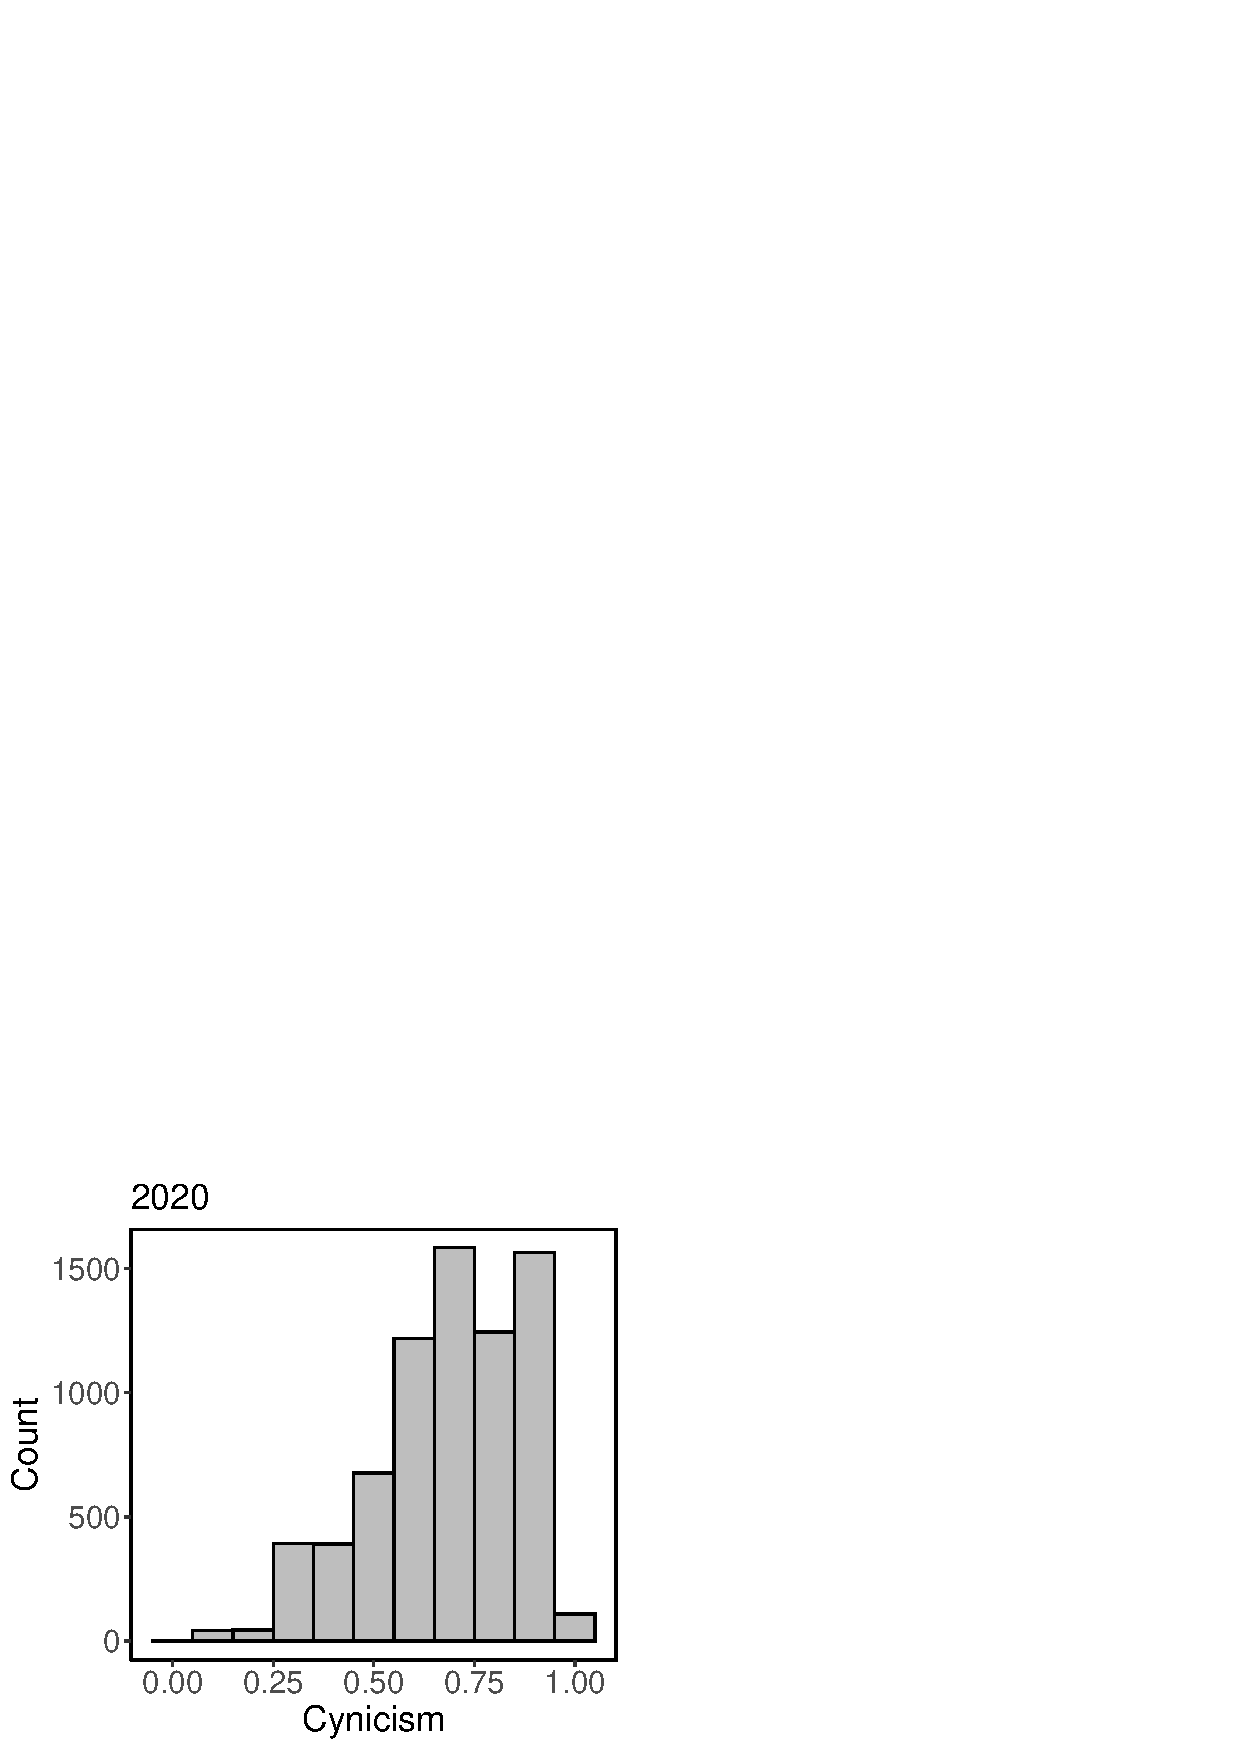
\includegraphics[width=\textwidth]{Figures/Descriptives-Histogram-Cynicism-2020.pdf}
        \end{subfigure}
        \begin{subfigure}[b]{0.4\textwidth}  
            \centering 
            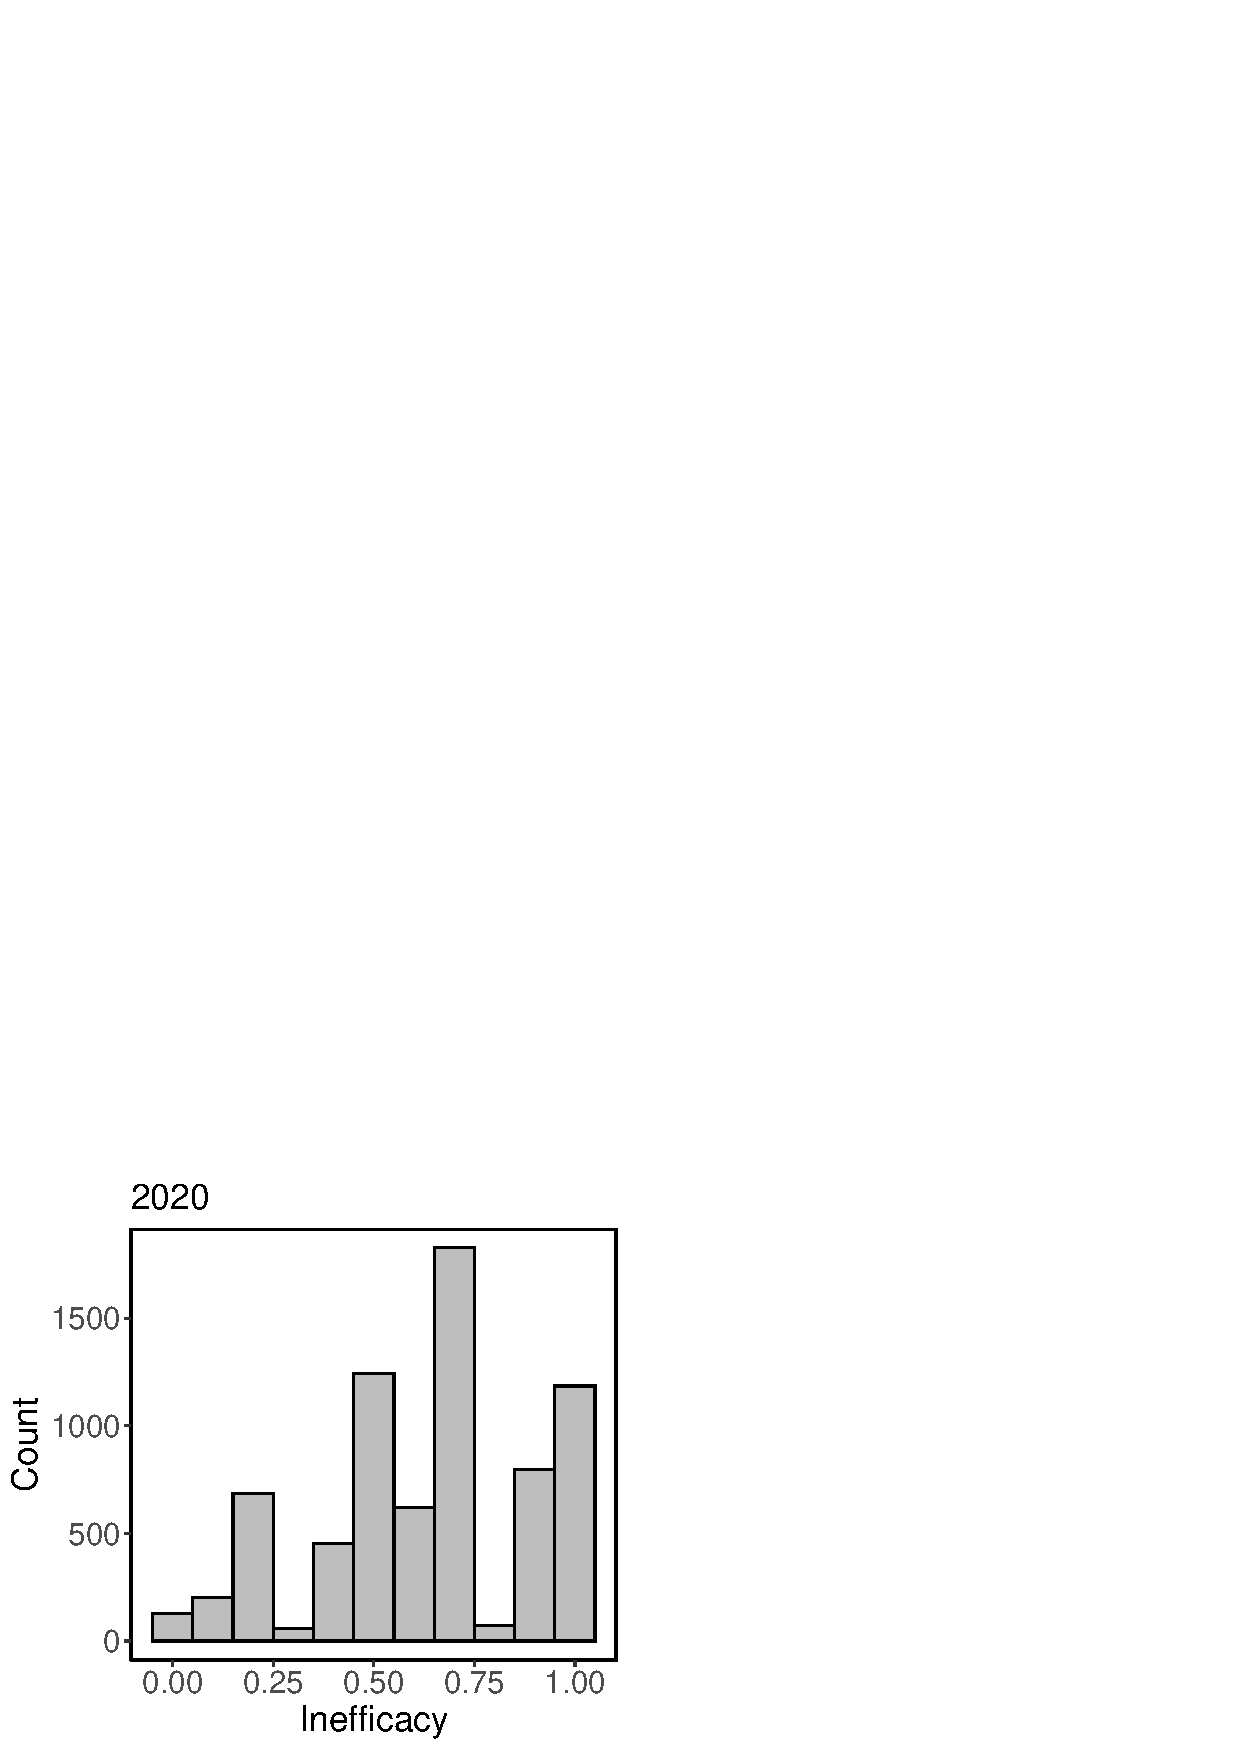
\includegraphics[width=\textwidth]{Figures/Descriptives-Histogram-Inefficacy-2020.pdf}
        \end{subfigure}
        
        \vskip\baselineskip
        \begin{subfigure}[b]{0.4\textwidth}   
            \centering 
            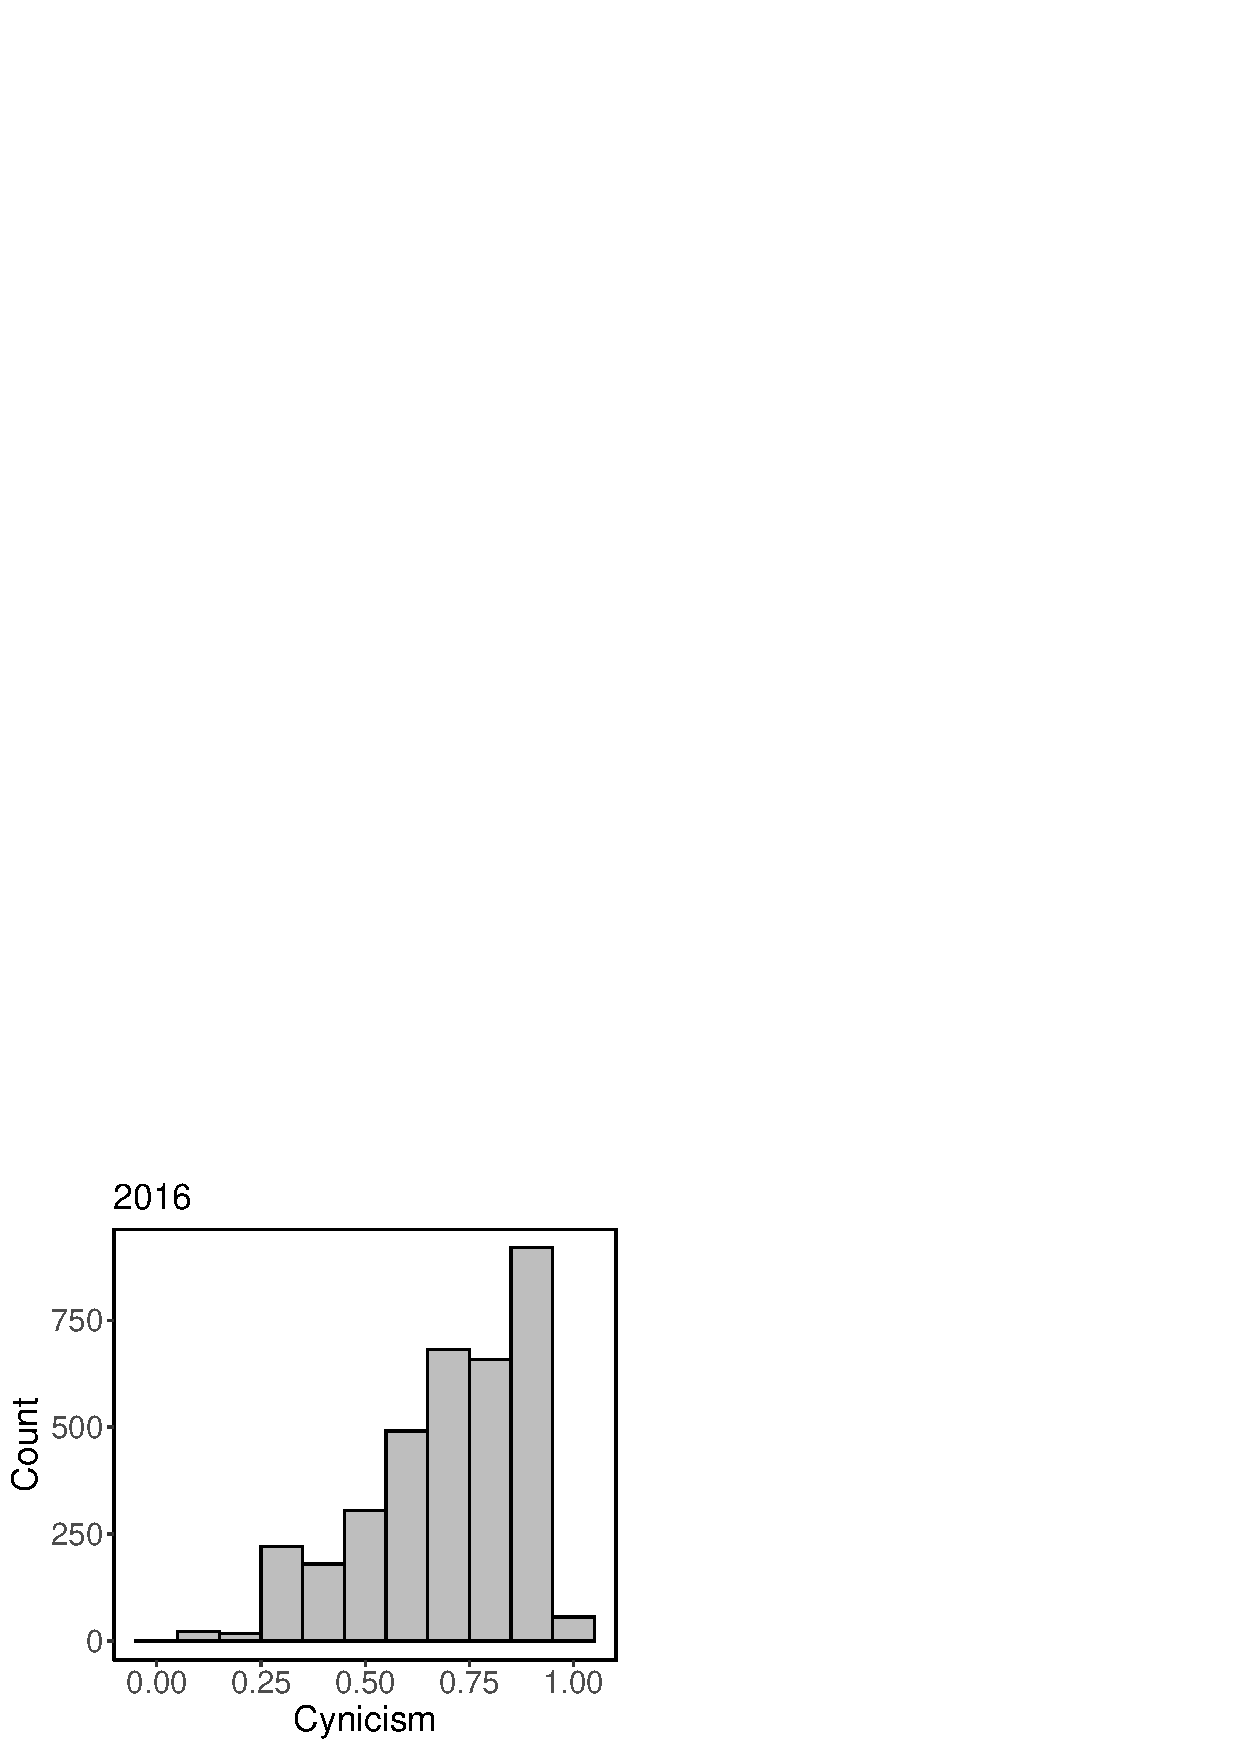
\includegraphics[width=\textwidth]{Figures/Descriptives-Histogram-Cynicism-2016.pdf}
        \end{subfigure}
        \begin{subfigure}[b]{0.4\textwidth}   
            \centering 
            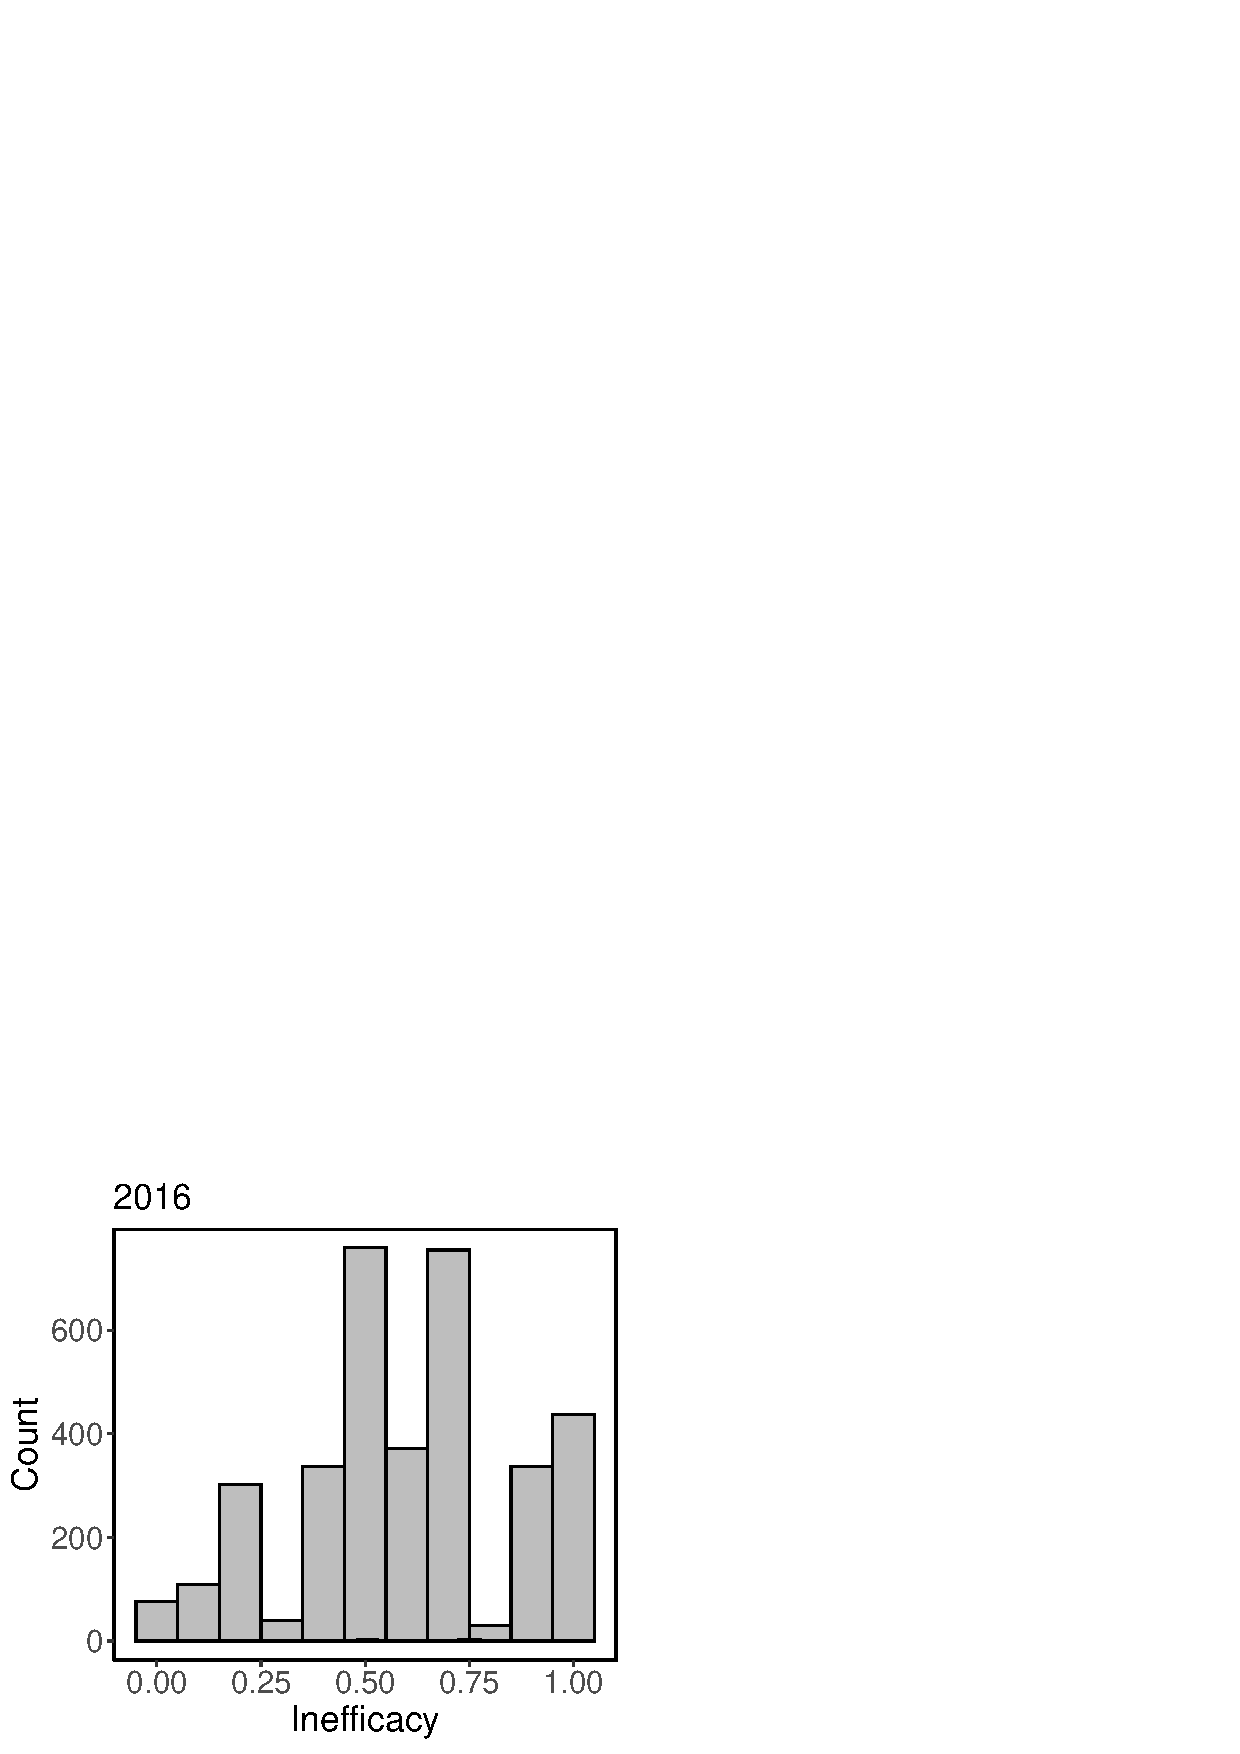
\includegraphics[width=\textwidth]{Figures/Descriptives-Histogram-Inefficacy-2016.pdf}
        \end{subfigure}
        
        \vskip\baselineskip
        \begin{subfigure}[b]{0.4\textwidth}   
            \centering 
            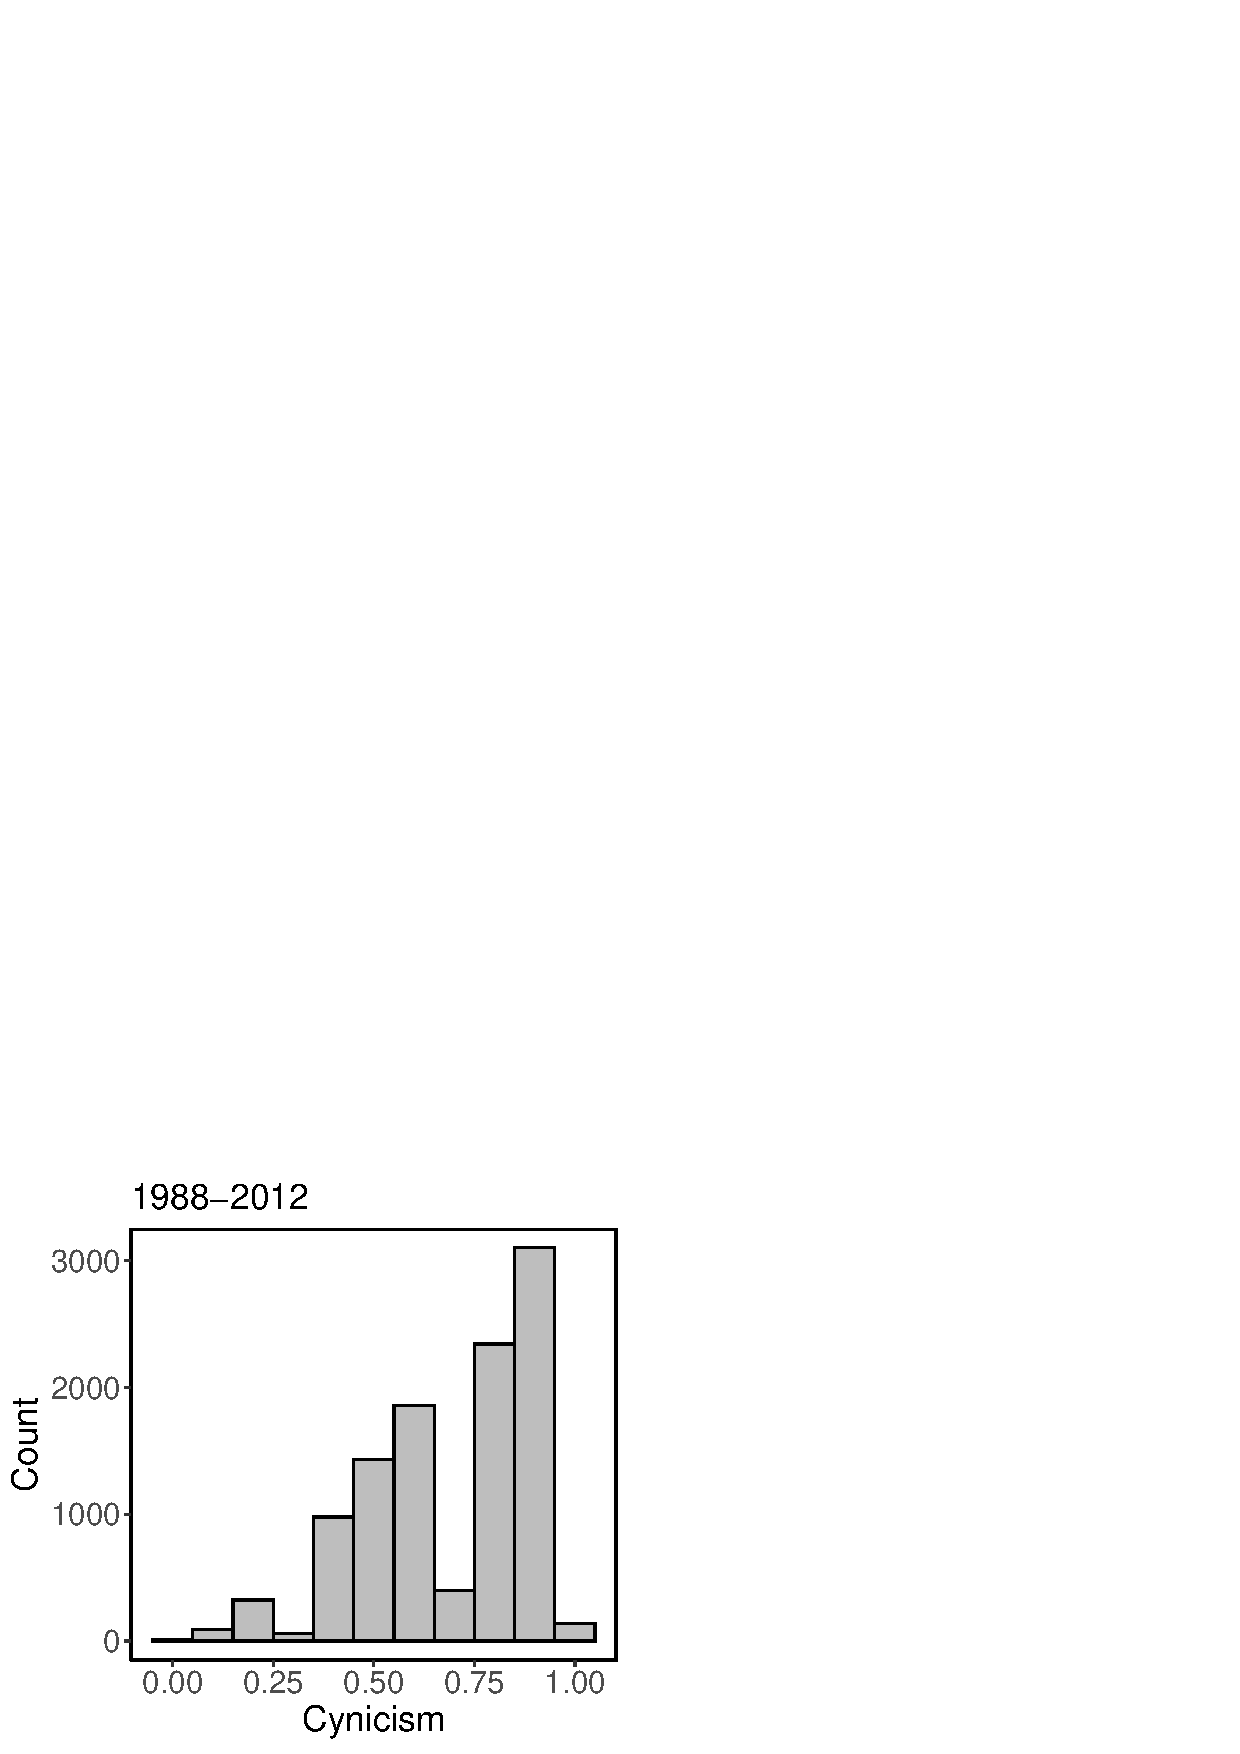
\includegraphics[width=\textwidth]{Figures/Descriptives-Histogram-Cynicism-CDF.pdf}
        \end{subfigure}
        \begin{subfigure}[b]{0.4\textwidth}   
            \centering 
            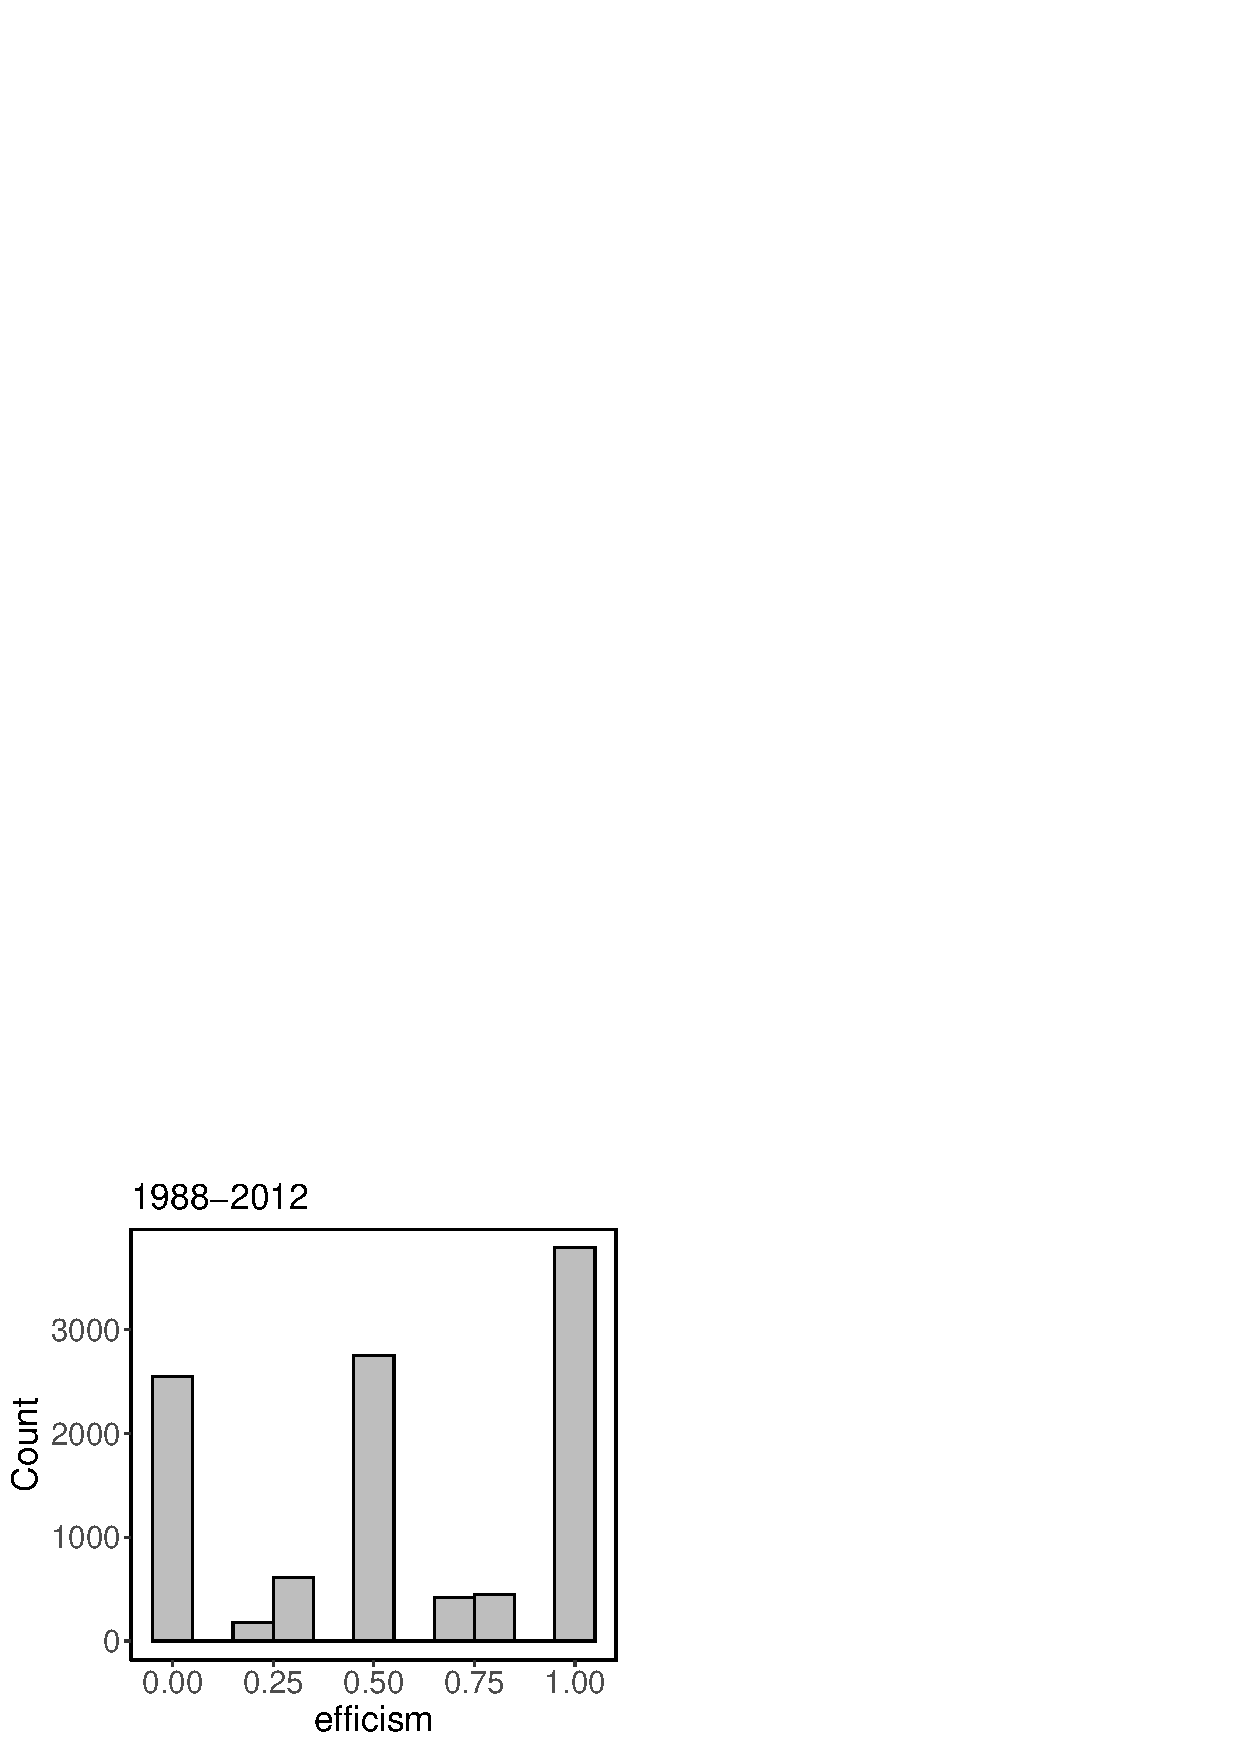
\includegraphics[width=\textwidth]{Figures/Descriptives-Histogram-Inefficacy-CDF.pdf}
        \end{subfigure}
        \caption{Histograms of Alienation Measures (Cynicism and Inefficacy)} 
        \label{fig:alienation-hists}
    \end{figure*}
    
   
    
\input{Tables/FA-Alienation-16-20.tex} % factor analysis of alienation items, 2016-2020
\input{Tables/FA-Alienation-88-12.tex} % factor analysis of alienation items, 1988-2012
\clearpage



\subsubsection{All Variables}\label{si:all-vars} % all variables

\input{Tables/Descriptives-20.tex} % descriptives, 2020
\input{Tables/Descriptives-16.tex} % descriptives, 2016
\input{Tables/Descriptives-88-12.tex} % descriptives, 1988-2012
\clearpage















%%%%%%%%%%%%%%%%%%%%%%%%%%%%%%%%%%%%%%%%%%%%%%%%%%%%
%%  %%%%%  %%%%%  %%%%%  %%%%%  %  %%%%%  %    %  %%
%%  %      %      %        %    %  %   %  % %  %  %%
%%  %%%%%  %%%%%  %        %    %  %   %  %  % %  %%
%%      %  %      %        %    %  %   %  %   %%  %%
%%  %%%%%  %%%%%  %%%%%    %    %  %%%%%  %    %  %%
%%%%%%%%%%%%%%%%%%%%%%%%%%%%%%%%%%%%%%%%%%%%%%%%%%%%
\section{Models}\label{si:mods}
All models handle missing data through list-wise deletion. This means that the number of observations in the models in Tables~\ref{tab:turnout-16} and \ref{tab:turnout-20} may decrease slightly as additional co-variates are introduced. 

% TURNOUT
\subsection{Turnout}\label{si:mods:turnout}
\input{Tables/Turnout-16-Mods.tex}
\input{Tables/Turnout-20-mods.tex}
\input{Tables/Turnout-16-20-Mods-Cyn-Eff-Separate.tex}
Communications with ANES staff in February of 2023 revealed that the sampling variables for the 1988-2020 ANES Time Series studies are not compatible through time (e.g., Cluster 1 in 2016 may not be the same as Cluster 1 in 1988). One option would be to create unique cluster-year and startum-year variables, but this would assume a level of independence between clusters through time, or stratum through time, that is not realistic or justifiable. Therefore, I estimate the model in Tables~\ref{tab:turnout-cyn-year-int} with weights, but not design-consistent standard errors, and assume that the standard errors I estimate likely understate variance. The results provide little evidence to support the claim I am attempting to test with these models anyway (i.e., compare the cynicism-turnout relationships in 2016 to previous years), so my decision to forego design-consistent standard errors is largely inconsequential. 

%\input{Tables/Turnout-88-12-Mods.tex}
\input{Tables/Turnout-88-12-Mods-Cyn-Int.tex}
\clearpage


% VOTE CHOICE
\subsection{Vote Choice}\label{si:mods:votechoice}
\input{Tables/VoteChoice-16-20-Mods.tex}
\clearpage






%%%%%%%%%%%%%%%%%%%%%%%%%%%%%%%%%%%%%%%%%%%%%%%%%%%%
%%  %%%%%  %%%%%  %%%%%  %%%%%  %  %%%%%  %    %  %%
%%  %      %      %        %    %  %   %  % %  %  %%
%%  %%%%%  %%%%%  %        %    %  %   %  %  % %  %%
%%      %  %      %        %    %  %   %  %   %%  %%
%%  %%%%%  %%%%%  %%%%%    %    %  %%%%%  %    %  %%
%%%%%%%%%%%%%%%%%%%%%%%%%%%%%%%%%%%%%%%%%%%%%%%%%%%%
\section{Structural Topic Model}\label{si:stm}

%% PRE-PROCESSING
\subsection{Pre-Processing}\label{si:preprocessing}
Before estimating Structural Topic Models on the open-ended responses about Trump, I started by pre-processing the texts which includes removing unnecessary punctuation, numbers, and stop words (e.g., ``it," ``what," ``is"), converting all characters to lowercase, translating any non-English responses to English, and correcting spelling. I also chose to remove terms that appear in no more than four documents and these words with contain little to no useful information for the model. Following these pre-processing steps, I am left with 4,724 documents and 982 terms in the corpus of texts about Trump.

%% MODEL SELECTION
\subsection{Model Selection}\label{si:modelselection}

\textcite{roberts2014stm} note that there is not necessarily a correct number of topics for any given corpus, so they recommend that researchers make this selection based on substantive knowledge that they many have about the content of the texts, and that they consider the purpose for which the texts will be used. Additionally, \textcite{roberts2019stm} provide the \texttt{searchK} function in their \texttt{stm} package to allow researchers a more empirically-driven method of selecting of the number of topics. Following this advice, I note that the 2008 ANES Likes/Dislikes about Candidates were manually coded by ANES staff into roughly 30 topics, so I expect roughly the same number of topics (or more) to be found in the 2016 responses about Trump. With this in mind, I proceed by using the \texttt{searchK} function to generate models that range in the number of topics from 30 to 40 topics. I generate performance diagnostics from these models such as held-out likelihood, residuals, semantic coherence, and lower bound and plot them in Figures~\ref{fig:selectingK}. 

In selecting the number of topics, we are looking for the semantic coherence and the held-out likelihood to be high while the residuals should be low. We see in Figure~\ref{fig:selectingK} that the model with 36 topics seems to provide the best balance of these criteria, so I set \textit{K} (i.e., the number of topics) to 36 in the model. Additionally, because the results of the STM are sensitive to initialization, the last step before finalizing the model is to use the \texttt{selectModel} function to generate several candidate models. From each of the model runs, I plot the semantic coherence and exclusivity, shown in Figure~\ref{fig:selectModel}. Notice that models 1 through 6 all show roughly the same values of semantic coherence and exclusivity. Because the models performed so similarly, I manually inspected the topic content from several of the models, and selected the model where the FREX (Frequent-Exclusive) words logically went together and a common theme could be discerned from exemplar texts. 


\begin{figure}[t!]
	\centering
	\includegraphics[width=0.8\textwidth]{Figures/STM-selectingK.pdf}
	\caption{Diagnostics for Determining the Number of Topics}
		\label{fig:selectingK}
\end{figure}


\begin{figure}[t!]
	\centering
	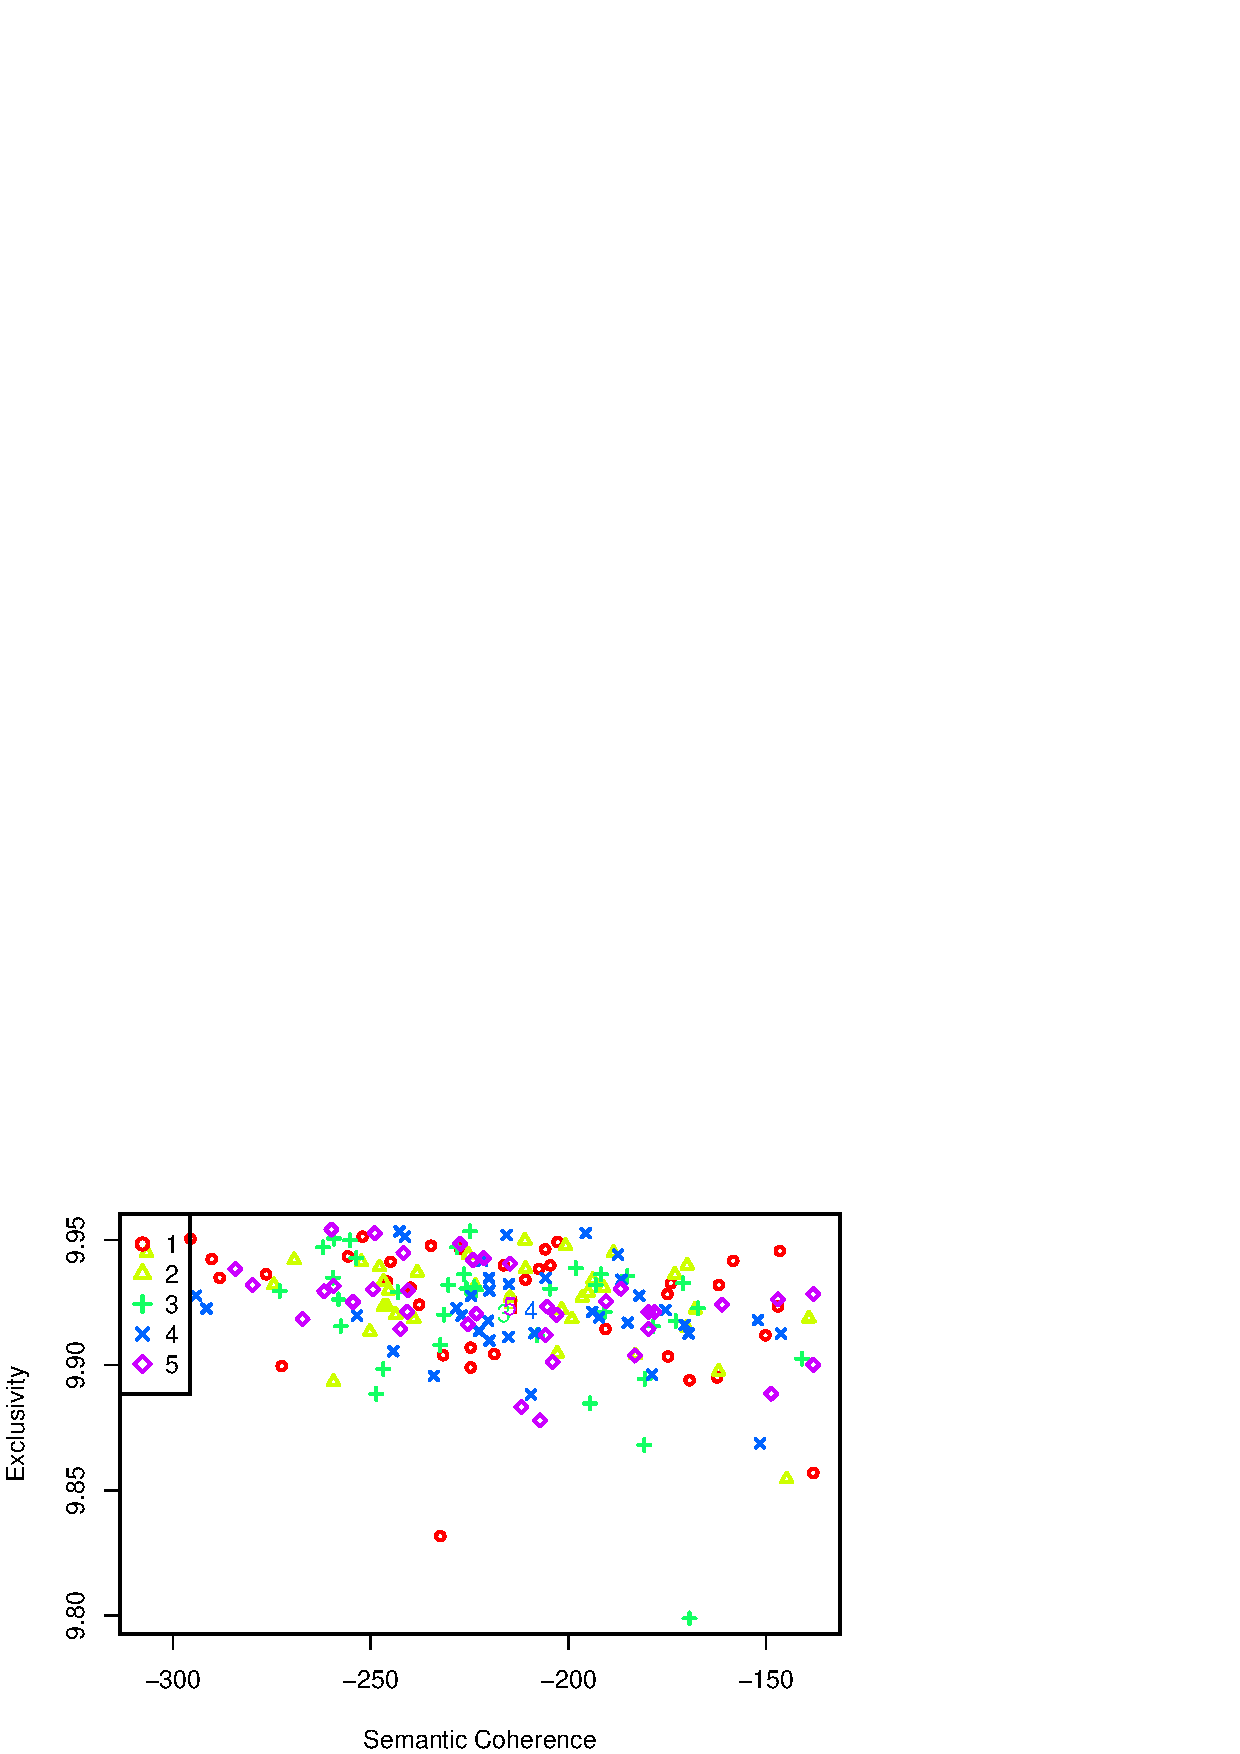
\includegraphics[width=0.8\textwidth]{Figures/STM-selectModel.pdf}
	\caption{Comparing Semantic Coherence and Exclusivity of Models with Various Initializations}\label{fig:selectModel}
\end{figure}


\clearpage
\begin{figure}[t!]
	\centering
	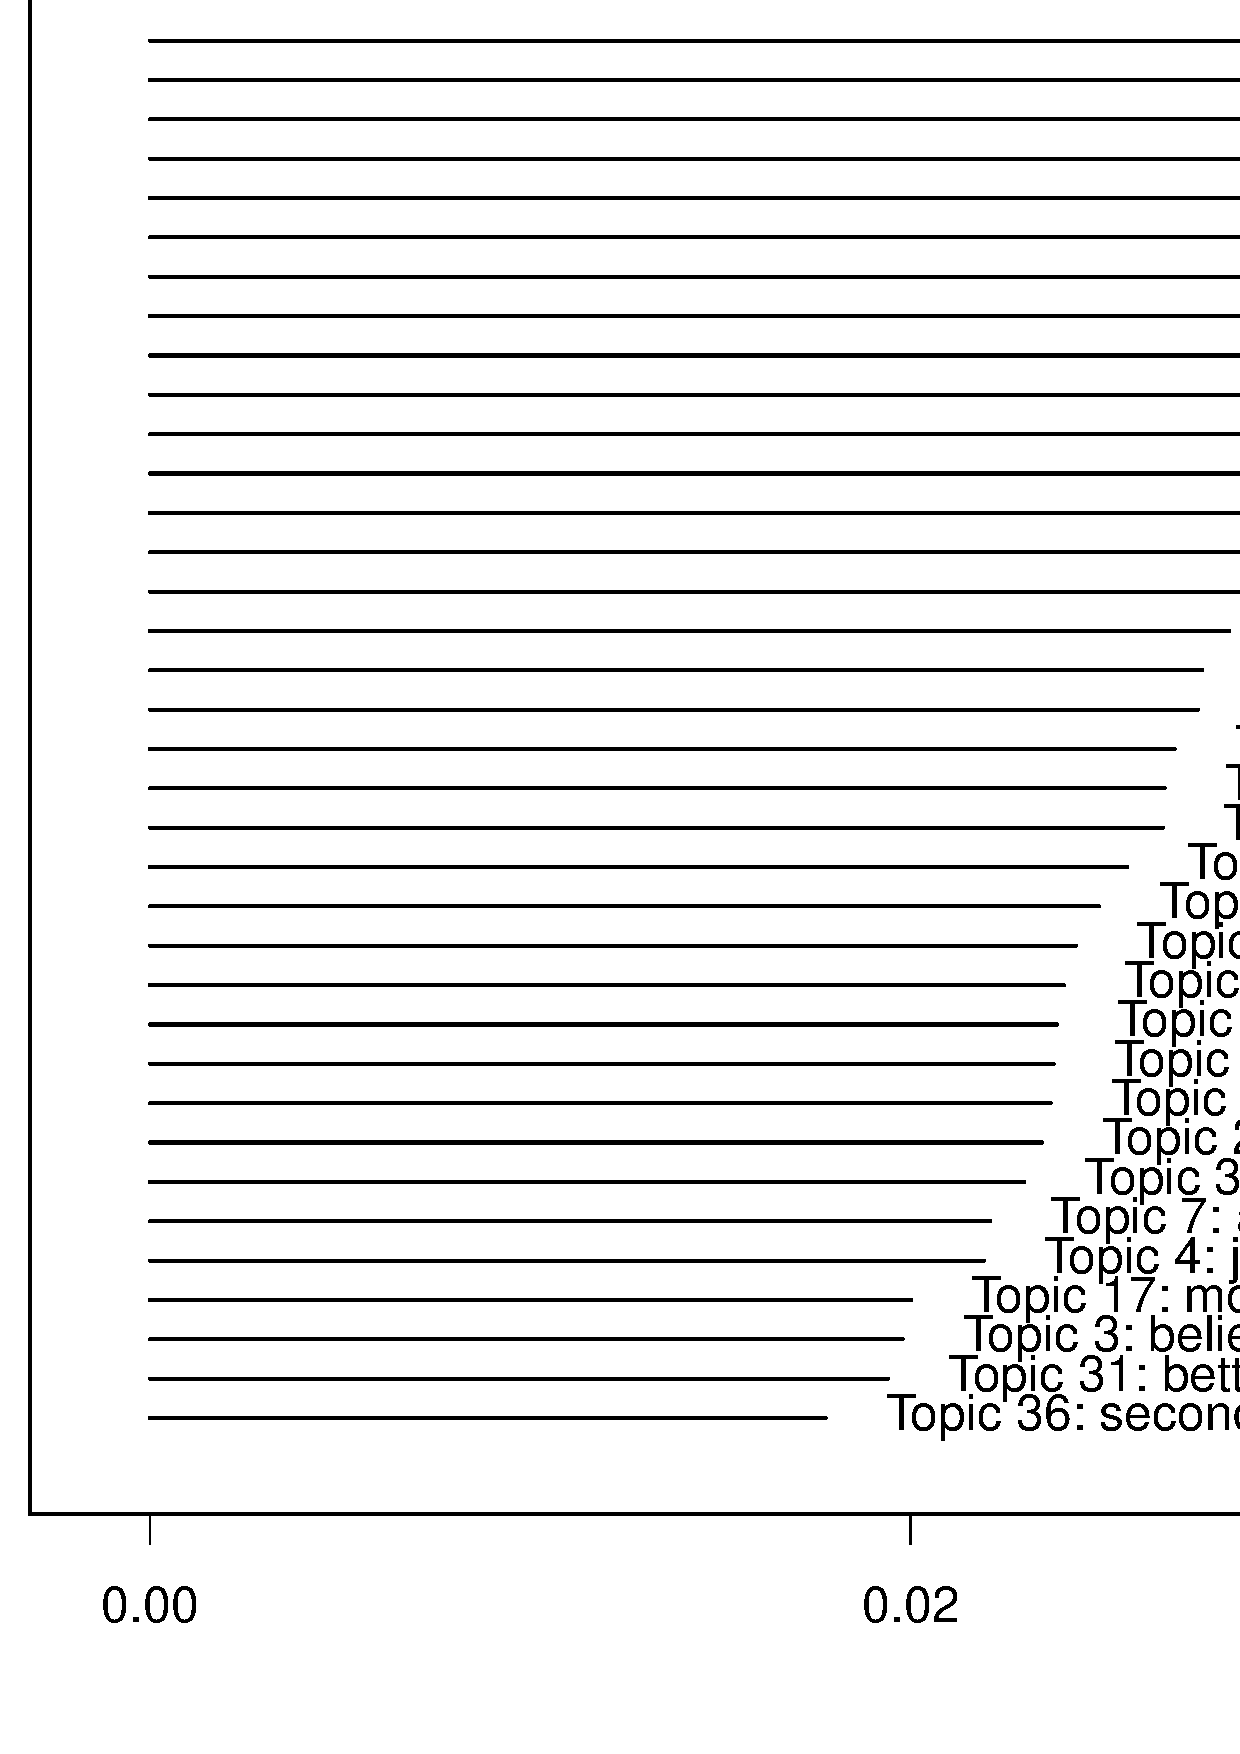
\includegraphics[width=0.95\textwidth]{Figures/STM-ExpectedTopicProportion.pdf}
	\caption{Expected Topic Proportion for All 36 Topics}
		\label{fig:alltopics}
\end{figure}


\clearpage
\subsection{Use of the ``Political Outsider" Topic}\label{si:stm-mods}
The built-in \texttt{estimateEffect} function from the \texttt{stm} package in R allows researchers to estimate the relationships between any predictors of interest and the use of particular topics from the model. Importantly, this function adjust standard errors to account for uncertainty in the estimation of the STM, but unfortunately it does not allow researchers to also include weights or account for complex sampling in the standard errors. Therefore, Column 1 of Table~\ref{tab:stm-mods} uses the \texttt{estimateEffect} function to predict use of the ``outsider'" topic across 2016 and 2020, while Column 2 uses the \texttt{svyglm} function from the \texttt{survey} package to incorporate weights and design-consistent standard errors.  The results are nearly identical. 

The 2016 ANES Time Series Study was conducted through both face-to-face interviews and web interviews, but due to the COVID-19 Pandemic, the 2020 ANES Time Series Study was forced to move entirely online. This creates the concern that the differences in the use of the ``outsider" topic that I am observing across the two elections is due to mode differences. I alleviate this concern by modeling only web responses from 2016 and 2020 in Column 3 of Table~\ref{tab:stm-mods}. The results with only the web sample are nearly identical to the full sample. 
\input{Tables/STM-Mods.tex}



\clearpage
\printbibliography
\end{refsection}
\end{appendices}










\end{document}